\chapter{Circumventing Undersegmentation - Joint Segmentation and Tracking}
\label{cha:joint}

Conservation tracking in conjunction with Gaussian mixture models is a powerful tool when it comes
to handling undersegmentation in the sense of multiple cells merged into a single foreground
object. Still, the overall result is strongly dependent on the segmentation. Another limitation is
the number of objects in a connected component being decided upon before the single objects are
reconstructed. The features of a single object are a strong indicator for the object being an actual
cell or clutter. This information cannot be taken into account in the conservation tracking
pipeline, as the number of objects in a connected component is inferred before
reconstruction. Furthermore, the existence of too many mergers, or mergers that cannot be resolved
due to the lack of a merging or demerging event, restrains the ability of the conservation tracking
algorithm to determine the correct number of cells within a connected
component. \cref{fig:joint-motivation-example} gives an example for data that requires a compromise
between segmenting as many cells as possible, even if close to background, and keeping the number
and size of merged objects low.

In order to circumvent the need for a compromise, we introduce a method for joint segmentation and
tracking in this thesis. This method additionally addresses lost cells that are close to
background. Instead of accepting a compromise as described above, the image needs to be
oversegmented in a sense that each cell is represented by at least one segment (also superpixel or
-voxel), and each segment cannot comprise more than one single cell. A probabilistic graphical model
then chooses -- with the help of global temporal information -- an appropriate final
segmentation. In contrast to conservation tracking with GMM, changing the segmentation is part of
the model and not only a post-processing operation. An overview as well as a detailed explanation of
each part of the algorithm are given in \crefrange{sec:joint-overview}{sec:joint-classifiers},
followed by experiments and results in \cref{sec:joint-experiments}.


\begin{figure}
    \centering
    \begin{subfigure}[t]{0.48\textwidth}
        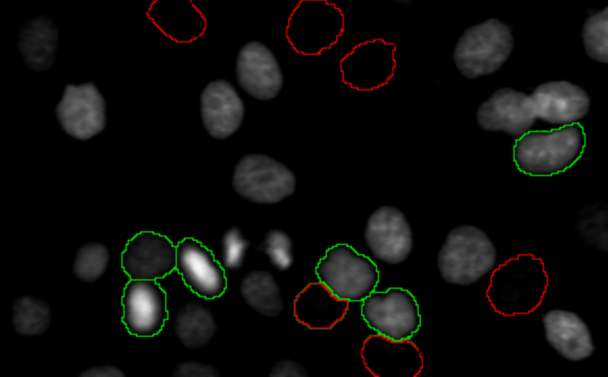
\includegraphics[width=\textwidth]{images/joint/mitocheck_255_max.pdf}
        \caption{This image shows raw data in its original intensity range $[0, 255]$. Cells that
            are close to background are not visible and are lost to the human observer
            (\cf~\cref{fig:joint-underseg-mergers}). This is equivalent to using only training
            examples that are distinct from background. Similar to the human observer, the
            classifier then will lose objects that are close to the background. Red color indicates
            cells that were lost in \cref{fig:joint-underseg-no-detection} while present in
            \cref{fig:joint-underseg-mergers}. In contrast, a green margin shows cells that are
            separated correctly in \cref{fig:joint-underseg-no-detection} while being merged in
            \cref{fig:joint-underseg-mergers}.}
        \label{fig:joint-underseg-no-detection}
    \end{subfigure}
    \hfill
    \begin{subfigure}[t]{0.48\textwidth}
        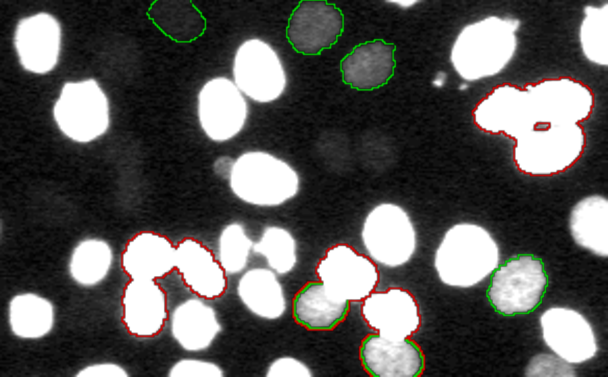
\includegraphics[width=\textwidth]{images/joint/mitocheck_030_max.pdf}
        \caption{Here, the image range $[0, 30]$ has been mapped to $[0, 255]$. In addition, any
            value greater than $30$ in the original image has been set to $255$. While this reveals
            many unseen cells, marked in green (red in \cref{fig:joint-underseg-no-detection}),
            it also produces more and larger mergers. Affected cells are enclosed in red, their
            counterparts in green in \cref{fig:joint-underseg-no-detection}. This
            corresponds to a segmentation classifier that is trained on near background cells as
            well. }
        \label{fig:joint-underseg-mergers}
    \end{subfigure}
    \caption[Undersegmentation in different segmentation approaches]{Illustration of the
        shortcomings of different segmentation approaches that both suffer from undersegmentation,
        based on data set C~(\cref{subsubsec:gmm-data-c}): either by losing many
        cells~(\subref{fig:joint-underseg-no-detection}) or by producing more and larger
        mergers~(\subref{fig:joint-underseg-mergers}). Examples for strengths and weaknesses of each
        approach are marked by green and red margins respectively.}
    \label{fig:joint-motivation-example}
\end{figure}

\section{Overview}
\label{sec:joint-overview}

Joint segmentation and tracking describes a method that breaks the fixed border between the
segmentation phase and the tracking phase in a
tracking-by-assignment~(\cref{sec:tracking-by-assignment}). More precisely, at first an
oversegmentation of the raw data is generated such that each foreground \emph{segment} contains not
more than a single cell. On the contrary, each cell in the raw data may consist of multiple
segments. The tracking model then decides whether a segment belongs to foreground or background and
groups segments into cell objects.

For clarity and an unambiguous definition of the joint segmentation and tracking, we first define
notational conventions that will be used throughout this chapter.
\begin{mydef}
    \label{def:joint-segment}
    A \emph{segment} or \emph{superpixel/-voxel} is the smallest unit in a segmentation. It is part of or a complete foreground
    object.
\end{mydef}

\begin{mydef}
    \label{def:joint-region}
    A \emph{region} is either a single segment or the union of two neighboring regions. Thus, the
    segments form a subset of all regions. Neighborhood relationships can be visualized in a
    \emph{region adjacency graph}.
\end{mydef}

\begin{mydef}
    \label{def:joint-conflict}
    Two regions \emph{contradict} each other if the intersection of their contained segments is not
    the empty set. In other words, they form a \emph{conflict}. These conflicts can be visualized in
    a conflict graph.
\end{mydef}

\begin{mydef}
    \label{def:joint-connected-component}
    A \emph{connected component} contains all segments that are connected by a path in the region
    adjacency graph.
\end{mydef}
Note that, by definition, a connected component is also a region. 

\begin{mydef}
    \label{def:joint-cardinality}
    The \emph{cardinality} of a region $r$ is the number of segments that the region consists of. It
    is denoted by $|r|$.
\end{mydef}
In the context of a conflict graph, the cardinality of a region $r$ is the number of maximal
cliques~(\cref{def:clique}) or \emph{``conflict sets''} in the conflict graph that contain region
$r$. In general, each conflict set contains exactly one segment, which can be used as an identifier
of the conflict set. These definitions are subsumed in \cref{tab:joint-definitions} with
illustrative visualizations.  \newlength\tablenormaltext
\settototalheight\tablenormaltext{\parbox{\linewidth}{Raw Data}}
\begin{table}
    \centering
    \scalebox{0.85}{
        \def\arraystretch{0.5}
% \setlength{\tabcolsep}{1pt}
\begin{tabularx}{\textwidth}{p{5cm}l}
    \toprule
    Definition  & Visualization \\ \midrule
    % \begin{minipage}[t]{0.15\linewidth}\small\vspace{-53pt}{$\begin{aligned}t&=75\\\id&=446\\
    %         k&=3\end{aligned}$}\end{minipage}&
    % \raisebox{-0.8\height{\includegraphics...}}
    Raw Data (original image \& enhanced contrast) &
    \raisebox{\tablenormaltext-\height}{
        
\includegraphics[width=0.18\textwidth]{images/joint/overseg/75/02/raw.png}}
    \raisebox{\tablenormaltext-\height}{
        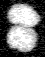
\includegraphics[width=0.18\textwidth]{images/joint/overseg/75/02/raw_contrast.png}} \\ & \\
    Segment&
    \raisebox{\tablenormaltext-\height}{
        
\includegraphics[width=0.18\textwidth]{images/joint/overseg/75/02/colored00.png}} \\ & \\
    Region (with ids) &
    \raisebox{\tablenormaltext}{
        \begin{tikzpicture}[baseline=(image1.north)]
            \node[anchor=south west,inner sep=0] (image1) {
                
\includegraphics[width=0.18\textwidth]{images/joint/overseg/75/02/colored00.png}};
            \begin{scope}[x={(image1.south east)},y={(image1.north west)}]
                \node[region_id] at (0.4, 0.75) {\huge{$1$}};
                \node[region_id] at (0.65, 0.7) {\huge{$2$}};
                \node[region_id] at (0.5, 0.32) {\huge{$3$}};
                % helpers
                % http://tex.stackexchange.com/questions/9559/drawing-on-an-image-with-tikz/9561
                % \draw[help lines,xstep=.1,ystep=.1] (0,0) grid (1,1);
                % \foreach \x in {0,2,...,8} { \node [anchor=north] at (\x/10,0) {0.\x}; }
                % \foreach \y in {0,2,...,8} { \node [anchor=east] at (0,\y/10) {0.\y}; }
            \end{scope}
        \end{tikzpicture}}
    \raisebox{\tablenormaltext}{
        \begin{tikzpicture}[baseline=(image2.north)]
            \node[anchor=south west,inner sep=0] (image2) {
                
\includegraphics[width=0.18\textwidth]{images/joint/overseg/75/02/colored01_all.png}};
            \begin{scope}[x={(image1.south east)},y={(image2.north west)}]
                \node[region_id] at (0.53, 0.73) {\huge{$4$}};
                \node[region_id] at (0.5, 0.32) {\huge{$3$}};
            \end{scope}
        \end{tikzpicture}}
    \raisebox{\tablenormaltext}{
        \begin{tikzpicture}[baseline=(image3.north)]
            \node[anchor=south west,inner sep=0] (image3) {
                
\includegraphics[width=0.18\textwidth]{images/joint/overseg/75/02/colored02.png}};
            \begin{scope}[x={(image1.south east)},y={(image3.north west)}]
                \node[region_id] at (0.5, 0.32) {\huge{$5$}};
            \end{scope}
        \end{tikzpicture}}
    \\ & \\
    Connected Component&
    \raisebox{\tablenormaltext-\height}{
        
\includegraphics[width=0.18\textwidth]{images/joint/overseg/75/02/colored02.png}} \\ & \\
    Region Adjacency Graph (edges indicate adjacency)&
    \raisebox{\tablenormaltext}{
        \begin{tikzpicture}[baseline=(r1.north)]
            \node[region_graph] (r1) {$1$};
            \node[region_graph, right=of r1.west] (r2) {$2$};
            \node[region_graph, below=of r1.north] (r3) {$3$};
            \node[region_graph, right=of r3.west] (r4) {$4$};
            \node[region_graph, right=of r2.west] (r5) {$5$};
            \path[region_edge] (r1) edge (r2);
            \path[region_edge] (r2) edge (r3);
            \path[region_edge] (r3) edge (r4);
        \end{tikzpicture}}
    \\ & \\
    Conflict Graph (edges indicate conflicts)&
    \raisebox{\tablenormaltext}{
        \begin{tikzpicture}[baseline=(r1.north)]
            \node[conflict_graph] (r5) {$5$};
            \node[conflict_graph, right=of r5.west] (r1) {$1$};
            \node[conflict_graph, below=of r5.north] (r2) {$2$};
            \node[conflict_graph, right=of r2.west] (r4) {$4$};
            \node[conflict_graph, left=of r2.east] (r3) {$3$};
            \path[conflict_edge] (r5) edge (r1);
            \path[conflict_edge] (r5) edge (r2);
            \path[conflict_edge] (r5) edge (r3);
            \path[conflict_edge] (r5) edge (r4);
            \path[conflict_edge] (r4) edge (r1);
            \path[conflict_edge] (r4) edge (r2);
        \end{tikzpicture}}
    \\ & \\
    \bottomrule
    
\end{tabularx}
\def\arraystretch{1.0}


%%% Local Variables: 
%%% mode: latex
%%% TeX-master: "../../main"
%%% End: 

    }
    \caption[Notational conventions in the joint segmentation and tracking]{Notational conventions in the joint segmentation and
        tracking with visualizations on a cell from data set
        C~(\cref{subsubsec:gmm-data-c}). Segments and regions are color coded for better
        distinguishability. In case of overlapping regions, multiple images are added.}
    \label{tab:joint-definitions}
\end{table}

With the definitions at hand, we now give a brief digest of our new joint segmentation and tracking
method. First, we obtain a possibly undersegmented partition of the raw data into foreground and
background. At this stage, a foreground connected component may contain more than one single
cell. Moreover, the segmentation aims to include all cells in the data into foreground, regardless
of possibly merged objects~(\cf \cref{fig:joint-underseg-mergers}). Then, another segmentation
algorithm is applied to the foreground mask of the data with the intent to
oversegment~(\cref{sec:joint-oversegmentation}). This divides the foreground into segments from which an
initial region adjacency graph is created. Next, regions are gradually merged to form a richer set of
\emph{segmentation hypotheses}. The \emph{tracking hypotheses graph} is then formulated on the
connected component in the image. An edge connecting two nodes $n_1$, $n_2$ in this graph means that
any pair of two regions, one from $n_1$ and one from $n_2$, is a potential tracking
assignment. Finally, a factor graph~(\cref{sec:joint-graphical-model}) is built on top of the
hypotheses graph. The factor graph incorporates prior belief on configurations inferred by local
classifiers~(\cref{sec:joint-classifiers}) as well as restrictions on possible assignments and
segmentation hypotheses that are defined by the conflict graph and the requirements of cell
tracking. Then, inference on this factor graph yields the optimal tracking solution. This procedure
is illustrated in \cref{fig:joint-pipeline}.

\begin{figure}
    \centering
    \scalebox{0.8}{
        \begin{tikzpicture}
    \newcommand{\distancebetween}{20}
    \newcommand{\shiftdistance}{100}
    \newcommand{\scalingfactor}{0.12}
    \newcommand{\halfscalingfactor}{\scalingfactor}
    
    \begin{scope}
        \begin{scope}[baseline=(raw2)]
    \begin{scope}[yshift=\distancebetween,
        every node/.append style={yslant=0.5,xslant=-1},
        yslant=0.5,xslant=-1]
        \node[inner sep=0, label={[xshift=5]above:{}}] (raw1) {
            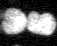
\includegraphics[width=\scalingfactor\textwidth]{images/joint/pipeline/78_raw_crop_enhanced.png}
        };
    \end{scope}
    \begin{scope}[every node/.append style={yslant=0.5,xslant=-1},yslant=0.5,xslant=-1]
        \begin{pgfonlayer}{bglower}
            \node[inner sep=0, label={[xshift=15]above:{}}] (raw2) {
                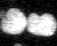
\includegraphics[width=\scalingfactor\textwidth]{images/joint/pipeline/79_raw_crop_enhanced.png}
            };
        \end{pgfonlayer}
    \end{scope}
    \coordinate (base1) at (raw2.north west |- raw2.south west);
    \coordinate (base2) at (raw2.south east |- raw2.south west);
    % \draw [pllbl]
    % (base1) -- (base2) node[black,midway,yshift=-0.6cm]
    % {Raw Data};
    \path let \p1 = (base1.west), \p2 = (base2.east) in
    node[pllbltxt, minimum width=\x2-\x1] (labelraw) at ($(base1)!0.5!(base2)$)
    {\phantom{g}Raw Data\phantom{g}};
    \begin{pgfonlayer}{bglower}
        \path[threed] (raw2.south east) -- (raw1.south east);
        \path[threed] (raw2.north east) -- (raw1.north east);
        \path[threed] (raw2.south west) -- (raw1.south west);
        \path[threed] (raw2.north west) -- (raw1.north west);
    \end{pgfonlayer}
\end{scope}

%%% Local Variables: 
%%% mode: latex
%%% TeX-master: "../../../main"
%%% End: 

        % \node[ultra thick, left=of raw1,yshift=5mm] {$t\phantom{+1}$};
        % \node[ultra thick, left=of raw2,yshift=5mm] {$t+1$};
        \begin{scope}[xshift=\shiftdistance, baseline=(seg2)]
    \begin{scope}[yshift=\distancebetween,
        every node/.append style={yslant=0.5,xslant=-1},
        yslant=0.5,xslant=-1]
        \node[inner sep=0, label={[xshift=5]above:{}}] (seg1) {
            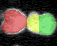
\includegraphics[width=\scalingfactor\textwidth]{images/joint/pipeline/78_seg_crop.png}
        };
    \end{scope}
    \begin{scope}[every node/.append style={yslant=0.5,xslant=-1},yslant=0.5,xslant=-1]
        \begin{pgfonlayer}{bglower}
            \node[inner sep=0, label={[xshift=15]above:{}}] (seg2) {
                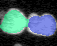
\includegraphics[width=\scalingfactor\textwidth]{images/joint/pipeline/79_seg_crop.png}
            };
        \end{pgfonlayer}
    \end{scope}
    \coordinate (base1) at (seg2.north west |- seg2.south west);
    \coordinate (base2) at (seg2.south east |- seg2.south west);
    % \draw [pllbl]
    % (base1) -- (base2) node[black,midway,yshift=-0.6cm]
    % {Initial Oversegmentation};
    \path let \p1 = (base1.west), \p2 = (base2.east) in
    node[pllbltxt, minimum width=\x2-\x1] (labelseg) at ($(base1)!0.5!(base2)$) {Oversegmentation};
    \begin{pgfonlayer}{bglower}
        \path[threed] (seg2.south east) -- (seg1.south east);
        \path[threed] (seg2.north east) -- (seg1.north east);
        \path[threed] (seg2.south west) -- (seg1.south west);
        \path[threed] (seg2.north west) -- (seg1.north west);
    \end{pgfonlayer}
\end{scope}

%%% Local Variables: 
%%% mode: latex
%%% TeX-master: "../../../main"
%%% End: 

        \begin{scope}[xshift=2*\shiftdistance, baseline=(cc2)]
    \begin{scope}[yshift=\distancebetween,
        every node/.append style={yslant=0.5,xslant=-1},
        yslant=0.5,xslant=-1]
        \node[inner sep=0, label={[xshift=5]above:{}}] (merge1) {
            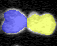
\includegraphics[width=\halfscalingfactor\textwidth]{images/joint/pipeline/78_merge_crop.png}
        };
        \node[inner sep=0,xshift=47,yshift=-47, label={[xshift=5]above:{}}] (cc1) {
            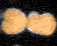
\includegraphics[width=\halfscalingfactor\textwidth]{images/joint/pipeline/78_cc_crop.png}
        };
    \end{scope}
    \begin{scope}[every node/.append style={yslant=0.5,xslant=-1},yslant=0.5,xslant=-1]
        \begin{pgfonlayer}{bglower}
            \node[inner sep=0, label={[xshift=15]above:{}},rectangle,thin,draw] (merge2) {
                \phantom{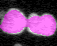
\includegraphics[width=\scalingfactor\textwidth]{images/joint/pipeline/79_cc_crop.png}}
            };
            \node[xshift=47,yshift=-47,inner sep=0, label={[xshift=15]above:{}}] (cc2) {
                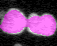
\includegraphics[width=\scalingfactor\textwidth]{images/joint/pipeline/79_cc_crop.png}
            };
        \end{pgfonlayer}
    \end{scope}
    \coordinate (base1) at (merge1.north west |- cc2.south west);
    \coordinate (base2) at (cc1.south east |- cc2.south west);
    % \draw [pllbl]
    % (base1) -- (base2) node[black,midway,yshift=-0.6cm]
    % {Region Merging};
    \path let \p1 = (base1.west), \p2 = (base2.east) in
    node[pllbltxt, minimum width=\x2-\x1] (labelmerging) at ($(base1)!0.5!(base2)$) {Region Merging};
    \begin{pgfonlayer}{bglower}
        \path[threed] (merge2.south east) -- (merge1.south east);
        \path[threed] (merge2.north east) -- (merge1.north east);
        \path[threed] (merge2.south west) -- (merge1.south west);
        \path[threed] (merge2.north west) -- (merge1.north west);

        \path[threed] (cc2.south east) -- (cc1.south east);
        \path[threed] (cc2.north east) -- (cc1.north east);
        \path[threed] (cc2.south west) -- (cc1.south west);
        \path[threed] (cc2.north west) -- (cc1.north west);
    \end{pgfonlayer}
\end{scope}

%%% Local Variables: 
%%% mode: latex
%%% TeX-master: "../../../main"
%%% End: 

        \begin{pgfonlayer}{background}
            \node[plbg, fit=(raw2.south west) (raw2.north west)
            (raw1.north east) (cc1.south east) (labelraw)] (bg1) {};
        \end{pgfonlayer}
        \draw[arrows=->, ultra thick, transform canvas={xshift=-15}] (bg1.north west) -- (bg1.south
        west) node[midway, xshift=-7] (t1) {\large{$t$}};
    \end{scope}
    \begin{scope}[yshift=-7.5*\distancebetween, xshift=100]
        \begin{scope}
    \begin{scope}[yshift=1.5*\distancebetween,
        every node/.append style={yslant=0.5,xslant=-1},
        yslant=0.5,xslant=-1]
        \node[inner sep=0] (image1) {
            \phantom{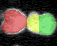
\includegraphics[width=\scalingfactor\textwidth]{images/joint/pipeline/78_seg_crop.png}}
        };
        \begin{pgfonlayer}{upper}
            \begin{scope}[every node/.append style={scale=0.7}]
                \node[fg_det, label={[font=\tiny]center:$X_1^t$}] (a1) at (image1.south east) {};
                \node[fg_det, label={[font=\tiny]center:$X_2^t$}] (a2) at ($(image1.south east)!0.5!(image1.north east)$) {};
                \node[fg_det, label={[font=\tiny]center:$X_3^t$}] (a3) at (image1.north east) {};
                \node[fg_det, label={[font=\tiny]center:$X_5^t$}] (a5) at ($(image1.south west)!0.5!(image1.north west)$) {};
                \node[fg_det, label={[font=\tiny]center:$X_4^t$}] (a4) at ($(a3)!0.5!(a5)$) {};
            \end{scope}
            \begin{scope}[every node/.append style={scale=0.5}]
                \node[conflict,yshift=-5] (c1) at ($(a1)!0.5!(a5)$) {};
                \node[conflict, right=of a3, xshift=-20, yshift=20] (c2) {};
                \node[conflict, yshift=-20] (c3) at (a4) {};
                \node[count, yshift=-20] (c4)  at ($(a2)!0.5!(a4)$) {};
                
                \path[count] (a1) edge (c4);
                \path[count] (a2) edge (c4);
                \path[count] (a3.south) edge (c4);
                \path[count] (a4) edge (c4);
                \path[count] (a5) edge[bend right=20] (c4);
                
                \path[conflict] (a5) edge[bend right=10] (c1);
                \path[conflict] (a1) edge (c1);

                \path[conflict] (a2) edge (c2);
                \path[conflict] (a4) edge[bend left=100] (c2);
                \path[conflict] (a5) edge[bend left=95] coordinate[pos=0.65](helpercoord1) (c2);

                \path[conflict] (a3) edge[bend left=10] (c3);
                \path[conflict] (a4) edge (c3);
                \path[conflict] (a5) edge (c3);
            \end{scope}
        \end{pgfonlayer}
        \begin{pgfonlayer}{bgupper}
            \node[rectangle, color=black,thick, fill=hypothesesbackground!30, opacity=0.8, draw=black,
            fit=(a1) (c2) (a5) (helpercoord1), inner sep=2, opacity=0.8, label={[xshift=5]above:{}}]
            (bgup) {};
        \end{pgfonlayer}
    \end{scope}
    \begin{scope}[every node/.append style={yslant=0.5,xslant=-1},yslant=0.5,xslant=-1]
        \node[inner sep=0] (image2) {
            \phantom{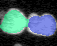
\includegraphics[width=\scalingfactor\textwidth]{images/joint/pipeline/79_seg_crop.png}}
        };
        \begin{pgfonlayer}{bglower}
            \node[rectangle, color=black,thick, fill=hypothesesbackground!30, opacity=0.8, draw=black,
            fit=(a1) (c2) (a5) (helpercoord1), inner sep=2, opacity=0.8, shift=($(image2) - (image1)$), label={[xshift=15]above:{}}]
            (bglow) {};
        \end{pgfonlayer}
        \begin{pgfonlayer}{lower}
            \begin{scope}[every node/.append style={scale=0.7}]
                \node[fg_det, label={[font=\tiny]center:$X_6^{t+1}$}] (b1) at (image2.south east) {};
                \node[fg_det, label={[font=\tiny]center:$X_7^{t+1}$}] (b2) at (image2.north east) {};
                \node[fg_det, label={[font=\tiny]center:$X_8^{t+1}$}] (b3) at ($(image2.south west)!0.5!(image2.north west)$) {};
            \end{scope}
            \begin{scope}[every node/.append style={scale=0.5}]
                \path[conflict] (b1) edge (b3);
                \path[conflict] (b3) edge (b2);
                \node[conflict] (c1) at ($(b1)!0.5!(b3)$) {};
                \node[conflict] (c2) at ($(b2)!0.5!(b3)$) {};
                \node[count] (c3) at ($(b1)!0.5!(b2)!0.3!(b3)$) {};
                \path[count] (b1) edge (c3);
                \path[count] (b2) edge (c3);
                \path[count] (b3) edge (c3);
            \end{scope}
        \end{pgfonlayer}
    \end{scope}
    \begin{pgfonlayer}{transition}
        \begin{scope}[every node/.append style={scale=0.6}]
            \node[fg_tra,label={[font=\tiny]center:$Y_{1,6}^t$},xshift=30] (trans1) at ($(a1)!0.55!(b1)$) {};
        \end{scope}
        \begin{scope}[every node/.append style={scale=0.2}]
            \node[transfac] (out) at ($(a1.center)!0.5!(trans1)$) {};
            \node[transfac] (in) at ($(b1.center)!0.5!(trans1)$) {};
            \path[transfac] (a1) edge (out.center);
            \path[transfac] (out) edge (trans1);
            \path[transfac] (trans1) edge (in);
            \path[transfac] (in) edge (b1.center);
        \end{scope}
    \end{pgfonlayer}
    \coordinate (base1) at (bglow.north west |- bglow.south west);
    \coordinate (base2) at (bglow.south east |- bglow.south west);
    % \draw [pllbl] (base1) -- (base2) node[black,midway,yshift=-0.6cm] {Factor Graph};
    \path let \p1 = (base1.west), \p2 = (base2.east) in
    node[pllbltxt, minimum width=\x2-\x1] (labelgraph) at ($(base1)!0.5!(base2)$) {Factor Graph};
    \begin{pgfonlayer}{bglower}
        \path[threed] (bglow.south east) -- (bgup.south east);
        \path[threed] (bglow.north east) -- (bgup.north east);
        \path[threed] (bglow.south west) -- (bgup.south west);
        \path[threed] (bglow.north west) -- (bgup.north west);
    \end{pgfonlayer}
\end{scope}

%%% Local Variables: 
%%% mode: latex
%%% TeX-master: "../../../main"
%%% End: 

        % \node[ultra thick, left=of raw1,yshift=5mm] {$t\phantom{+1}$};
        % \node[ultra thick, left=of raw2,yshift=5mm] {$t+1$};
        \begin{scope}[xshift=1.3*\shiftdistance]
    \begin{scope}[yshift=\distancebetween,
        every node/.append style={yslant=0.5,xslant=-1},
        yslant=0.5,xslant=-1]
        \node[inner sep=0, label={[xshift=5]above:{}}] (res1) {
            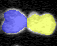
\includegraphics[width=\scalingfactor\textwidth]{images/joint/pipeline/78_res_crop.png}
        };
    \end{scope}
    \begin{scope}[every node/.append style={yslant=0.5,xslant=-1},yslant=0.5,xslant=-1]
        \begin{pgfonlayer}{bglower}
            \node[inner sep=0, label={[xshift=15]above:{}}] (res2) {
                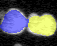
\includegraphics[width=\scalingfactor\textwidth]{images/joint/pipeline/79_res_crop.png}
            };
        \end{pgfonlayer}
    \end{scope}
    \coordinate (base1) at (res2.north west |- bglow.south west);
    \coordinate (base2) at (res2.south east |- bglow.south west);
    % \draw (base1) rectangle[pllbltxt, yshift=-10] (base2);%  {Tracking Result};
    \path let \p1 = (base1.west), \p2 = (base2.east) in
    node[pllbltxt, minimum width=\x2-\x1]  (labelres) at ($(base1)!0.5!(base2)$) {Tracking Result};
    \begin{pgfonlayer}{bglower}
        \path[threed] (res2.south east) -- (res1.south east);
        \path[threed] (res2.north east) -- (res1.north east);
        \path[threed] (res2.south west) -- (res1.south west);
        \path[threed] (res2.north west) -- (res1.north west);
    \end{pgfonlayer}
\end{scope}

%%% Local Variables: 
%%% mode: latex
%%% TeX-master: "../../../main"
%%% End: 

        \begin{pgfonlayer}{background}
            \node[plbg, fit=(bglow.south west) (bglow.north west)
            (bgup.north east) (res1.south east) (labelres.south)] (bg2) {};
        \end{pgfonlayer}
        \draw[arrows=->, ultra thick, transform canvas={xshift=-15}] (bg2.north west) -- (bg2.south
        west) node[midway, xshift=-7] (t2) {\large{$t$}};
    \end{scope}

    \begin{pgfonlayer}{background}
        \coordinate[xshift=0mm,left=of t1] (hawaii);
        \coordinate[right=of bg1.east,xshift=0mm] (coordeast);
        % \coordinate[below right=of bg1.south east,yshift=-5mm] (coordsouth);
        \coordinate (helper) at ($(bg1.south)!0.5!(bg2.north)$);
        \coordinate (coordsoutheast) at (coordeast |- helper);
        \coordinate[left=of t2.west,xshift=0mm] (coordwestwest);
        \coordinate[xshift=15mm] (coordwest) at (coordwestwest);
        \coordinate (coordsouthwest) at (coordwestwest |- helper);
        \path[arrows=->,draw, line width=4mm, color=red!40, rounded corners=5pt] (hawaii) -- (bg1.east) -- (coordeast) --
(coordsoutheast) -- (coordsouthwest) -- (coordwestwest) -- (coordwest) -- (coordeast |- bg2.east);
    \end{pgfonlayer}
    
\end{tikzpicture}

%%% Local Variables: 
%%% mode: latex
%%% TeX-master: "../../../main"
%%% End: 

    }
    \caption[Joint segmentation and tracking pipeline]{Joint segmentation and tracking
        pipeline. First, an initial oversegmentation is generated from raw data. Then, a richer set
        of segmentation hypotheses is created by merging existing regions. Note that the empty frame
        at the later time step indicates that there is no intermediate region merging as the
        connected component consists of only two segments and merging them results in the connected
        component. The factor graph models assignment hypotheses and incorporates cell tracking and
        consistency constraints. Finally, MAP inference on the factor graph yields the tracking
        result.}
    \label{fig:joint-pipeline}
\end{figure}

After an in depth introduction to the proposed method in
\crefrange{sec:joint-oversegmentation}{sec:joint-classifiers}, \cref{sec:joint-experiments} shows
experimental results. Note that the proposed method is equivalent to chain graph tracking
(\cref{subsec:fg-chaingraph}) with learned factors in case of single object connected components,
\ie each connected component contains exactly one segment.

%%% Local Variables: 
%%% mode: latex
%%% TeX-master: "../../../main"
%%% End: 

\section{Oversegmentation}
\label{sec:joint-oversegmentation}

The oversegmentation in the joint tracking and segmentation model follows a three-step procedure:
\begin{enumerate}
    \item Obtain a partition into foreground and background such that as many cells as possible are
  included -- not necessarily as single objects -- in the foreground~(\cref{subsec:joint-undersegmentation}).
    \item Partition the foreground mask into segments with the aim of an oversegmentation of all
  contained cells~(\cref{subsec:joint-oversegmentation}).
    \item Form a richer set of segmentation hypotheses by gradually merging segments into larger
  regions~(\cref{subsec:joint-region-merging}).
\end{enumerate}
In the following, we give a detailed description of our approach towards each of these tasks and the
generation of the hypotheses graph. Note that, in general, it is possible to exchange our approach
with a suitable replacement at any point of the three-step procedure.

\subsection{Initial Partitioning}
\label{subsec:joint-undersegmentation}
In general, the initial partitioning of the data into foreground and background follows the
procedure of the segmentation in the chain graph~(\cref{subsec:fg-chaingraph}) and
conservation~(\cref{subsec:fg-conservation}) tracking methods. First, a random forest
classifier~(\cref{cha:app-rf}) is trained on a small number of user annotated training samples using
ILASTIK~\citep{sommer_11_ilastik}. Then, the classifier predicts \emph{probability maps} for the
complete data set which can be transferred into a partitioning into foreground and background by
thresholding on the foreground probability of each pixel.

Contrary to the previous methods, chain graph and conservation tracking, the initial partitioning is
only the basis for another segmentation and thus we do not aim for a segmentation that has a
bijective mapping from cells in the raw data to foreground connected components. In fact, the
foreground includes as many cells as possible, even if they are merged into large connected
components.

\subsection{Oversegmentation}
\label{subsec:joint-oversegmentation}
Now an oversegmentation of the foreground mask is generated. To this end, the watershed
algorithm~\citep{vincent_91_watersheds,roerdink_00_watershed} is applied to the inverse of
the distance transform~\citep[Section~18.4.4]{jaehne_05_digital} of the foreground regions with seeds
at the local maxima of the distance transform, \ie the points on the foreground mask which are
locally furthest away from any background region. This gives rise to regularly shaped compact
segments, potential cell segmentations, which are the nodes of the initial region adjacency
graph. For each pair of conterminous regions, an edge between the corresponding nodes is added to
the graph.

\subsection{Region Merging}
\label{subsec:joint-region-merging}
Starting from the initial region adjacency graph, regions are merged into a richer set of possibly
competing cell segmentation hypotheses. For simplicity, we choose a hierarchical region merging with
$L$ levels. However, any region merging algorithm is applicable. The weight $w$ of an edge $E$
between two nodes $r_1$, $r_2$ in the region adjacency graph is a similarity measure for neighboring
regions based on the joint border of the involved regions. At each level $1 \le l \le L$ all pairs of
regions with similarity greater than a threshold $\tau$,
\begin{align}
    w(r_1, r_2) \ge \tau,
\end{align}
are merged into a new region. In the region adjacency graph, the two corresponding nodes are
contracted.

% \begin{figure}
%     \centering
%     \begin{subfigure}{0.48\textwidth}
%         \centering
%         \begin{tikzpicture}[baseline=(image1.north)]
    \node[anchor=south west,inner sep=0] (image1) {
        
\includegraphics[width=0.7\textwidth]{images/joint/overseg/75/02/colored00.png}};
    \begin{scope}[x={(image1.south east)},y={(image1.north west)}]
        \node[region_id] (r1) at (0.4, 0.75) {\huge{$1$}};
        \node[region_id] (r2) at (0.65, 0.7) {\huge{$2$}};
        \node[region_id] (r3) at (0.5, 0.32) {\huge{$3$}};
        \node[rectangle, draw, fit=(r1) (r2), color=green,line width=2pt, inner sep=8mm] (f) {};
        % helpers
        % http://tex.stackexchange.com/questions/9559/drawing-on-an-image-with-tikz/9561
        % \draw[help lines,xstep=.1,ystep=.1] (0,0) grid (1,1);
        % \foreach \x in {0,2,...,8} { \node [anchor=north] at (\x/10,0) {0.\x}; }
        % \foreach \y in {0,2,...,8} { \node [anchor=east] at (0,\y/10) {0.\y}; }
    \end{scope}
\end{tikzpicture}


%%% Local Variables: 
%%% mode: latex
%%% TeX-master: "../../../main"
%%% End: 

%         \caption{Regions $1$ and $2$ are similar and therefore merging is preferable.}
%     \end{subfigure}
%     \hfill
%     \begin{subfigure}{0.48\textwidth}
%         \centering
%         \begin{tikzpicture}[baseline=(image2.north)]
    \node[anchor=south west,inner sep=0] (image2) {
        
\includegraphics[width=0.7\textwidth]{images/joint/overseg/75/02/colored01_all.png}};
    \begin{scope}[x={(image1.south east)},y={(image2.north west)}]
        \node[region_id] (r4) at (0.53, 0.73) {\huge{$4$}};
        \node[region_id] (r3) at (0.5, 0.32) {\huge{$3$}};
        \node[rectangle, draw, fit=(r3) (r4), color=red,line width=2pt, inner sep=9.3mm, text
        width=5em, yshift=-0.7mm] (f) {};
    \end{scope}
\end{tikzpicture}

%%% Local Variables: 
%%% mode: latex
%%% TeX-master: "../../../main"
%%% End: 

%         \caption{The union of regions $3$ and $4$ is unlikely to be a cell. Therefore, the
%             similarity is low.}
%     \end{subfigure}
%     \caption[Different edge weights]{Edge weights between different pairs of region indicated by the
%     color of the circumscribing rectangle: green and red indicate high and low similarity respectively.}
%     \label{fig:joint-overseg-edge-weight}
% \end{figure}

By construction, regions potentially contradict each other. These conflicts are graphically
represented by the conflict graph $G_{\text{con}}$ with a node for each region and an edge for each
pair of regions which share at least one common segment:
\begin{align}
    G_{\text{con}} &= (\mathcal{V}_{\text{con}}, \mathcal{E}_{\text{con}}), \\
    \mathcal{E}_{\text{con}} &= \{V_1 \undirected V_2  : r_{V_1} \cap r_{V_2} \ne \emptyset\}.
\end{align}

\subsection{Hypotheses Graph}
\label{subsec:joint-hypotheses-graph}
In contrast to the chain graph method, the hypotheses graph of the joint segmentation and tracking
does not contain single detection and transition hypotheses. In fact, each node represents a
connected component and thus contains as many segmentation hypotheses as there are regions within
that connected component. In a similar fashion, the edges represent all possible transitions between
regions in the respective connected components.  Likewise to the chain graph hypotheses graph, edges
between connected components are determined by a nearest neighbor search. In practice, however, a
restriction on the number of possible transitions advisable in order to reduce the model size. To
this end, assignment hypotheses are generated only between all regions in each conflict set in a
connected component $c^t$ at time $t$ and all regions in the nearest neighbor conflict set for each
connected component $c^{t+1}$ at time $t+1$ with an edge $c^t \undirected c^{t+1}$ in the hypotheses
graph. In this context, the distance between two conflict sets is measured by the Euclidean distance
between the two segments that define these conflict sets. As a result of this \emph{pruning},
regions that are further up in the segmentation hierarchy have more potential assignments, with the
outgoing assignments of a connected component being not affected by the pruning. Finally, a factor
graph is constructed from the hypotheses graph.

% Before joint segmentation and tracking becomes computationally feasible, 
% the time-series of 2D/3D images/volumes need to be preprocessed
% to reduce the problem space (step (II) and (III) in \cref{fig:pipeline}). 
% Here, the images are processed each independently which allows for
% paralellization of the oversegmentation algorithm. 
% In step (II), the purpose is to obtain an oversegmentation on every image 
% which is sufficiently fine but as coarse as possible.
% That is, we prefer single segments (superpixels) for (isolated) objects without
% ambiguities, whereas multiple (smaller) segments are desired in cases where objects overlap in space. 

% To this end, we propose the following oversegmentation algorithm:
% \begin{enumerate}
%  \item Obtain a coarse segmentation which only distinghuishes 
% potential foreground from certain background.
%  \item Automatically select seeds fulfilling the requirements outlined above.
%  \item Compute the seeded watershed on the foreground mask.
%  \item Merge resulting segments hierarchically to potential regions.
% \end{enumerate}

% Here, the first step may be performed by any segmentation algorithm which can be adjusted in a way that 
% only those pixels/voxels are predicted as background where we are most sure. This step's output
% is either a hard segmentation or a probability map of the foreground (soft segmentation). 
% Note that typically, it is not desirable to track the resulting connected components directly, since 
% large clusters of cells may be contained in each connected component. Hence, we continue by 
% refining these connected components to multiple segments.

% To this end, the watershed algorithm is applied to the mask of potential foreground (``\emph{foreground mask}'').
% The seeds for it are determined by the local maxima of the distance transform on the foreground mask
% to nearest background pixels/voxels. This gives rise to regularly shaped compact segments, potential cell segmentations. 
% A minimum
% size of these segments may be achieved by performing a dilation operation on the seeds with appropriate disc radius.
% Note that the watershed may either be applied to the \emph{soft} segmentation mask or the masked raw data directly.

% Finally, segments are merged to regions, possible competing cell segmentations (step (III) in \cref{fig:pipeline}).  
% This merging can be performed in any order, but
% for simplicity, we choose a hierarchical region merging in a region adjacency graph using $L$ levels. 
% Its edge weights between neighboring segments/regions may be arbitrary complex and the regions may be merged 
% in an order determined by these edge weights.

% Since the (merged) regions will spatially overlap with their original segments, natural conflicts between 
% these regions exist and are incorporated into our graphical model (step (IV) in \cref{fig:pipeline})
% as discussed in the next section.


%%% Local Variables: 
%%% mode: latex
%%% TeX-master: "../../../main"
%%% End: 

\section{Graphical Model}
\label{sec:joint-graphical-model}
\begin{figure}
\begin{center}
    \begin{tikzpicture}[auto, thick, on grid,scale=1.8,every node/.style={scale=1.5, thick}]
        % Physical layer nodes

\newcommand{\distancebetween}{80}

\begin{scope}[
    yshift=\distancebetween,
    every node/.append style={yslant=0.5,xslant=-1},yslant=0.5,xslant=-1
    ]
    \begin{pgfonlayer}{upper}
        % \draw[black,thin, fill=black!70!blue, opacity=1, fill opacity=0.2] (-3,1.0) rectangle (0.1,3.2);
        \foreach \place/\x/\id/\t in {{(-2.7,2.9)/1/1/1}, {(-2.7,2.1)/2/2/1},{(-0.2,2.1)/3/5/1},
            {(-2.7,1.3)/4/3/1}, {(-1.25,1.7)/5/4/1}} {
            \node[hypotheses_three_objects, draw=blue!100, fill=blue!10, label=center:\footnotesize{$\displaystyle X_{\id}^{\t}$},
            ultra thick] (a\x) at \place {\phantom{\small{0}}};
        }

        % \node[unaryfac, above of=a3,yshift=-3mm,label=above right:$\psi_{\text{det}}$] (u1) {};
        % \path[unaryfac] (a3) edge (u1);
        % \node[unaryfac, below right of=a5,xshift=-2.2mm,yshift=2.2mm)] (u2) {};
        % \path[unaryfac] (a5) edge (u2);
        % \node[unaryfac, above left of=a1,yshift=-3mm] (u3) {};
        % \path[unaryfac] (a1) edge (u3);
        % \node[unaryfac, above left of=a2,yshift=-3mm] (u4) {};
        % \path[unaryfac] (a2) edge (u4);
        % \node[unaryfac, above left of=a4,yshift=-3mm] (u5) {};
        % \path[unaryfac] (a4) edge (u5);

        % \coordinate[draw=black!0, left of=a4] (helper1) {};
        % \coordinate[draw=black!0, left of=a3] (helper2) {};
        % \coordinate[draw=black!0, left of=helper2] (helper3) {};
        \node[conflict, left of=a4] (helper1) {};
        \node[conflict, left of=a3, xshift=1mm] (helper2) {};
        \node[conflict, yshift=5, label=above right:$\psi_{\text{det}}$] (helper4) at ($(a1)!0.5!(a3)$) {};
        \node[count, left of=helper2] (helper3) {};
        
        % Physical layer links
        \path[conflict] (a1) edge[bend left=0] (helper4);
        \path[conflict] (helper4) edge[bend left=0] (a3);
        \path[conflict] (a5) edge (helper2);
        \path[conflict, bend left=10] (a4) edge (helper2);
        
        \path[conflict] (a5) edge[bend left=50] (helper1);
        \path[conflict] (helper1) edge[bend left=50] (a2.west);

        \path[conflict] (a3) edge[bend left=60] coordinate[pos=0.65](helpercoord1) (helper1);
        % \gettikzxy{(helpercoord1)}{\ax}{\ay}; \coordinate (newfit) at (\ax,\ay);
        % \path[thick,black] (helpercoord1) edge (helper1);
        \path[conflict] (a3) edge (helper2);

        \path[count] (a1) edge (helper3);
        \path[count] (a2) edge (helper3);
        \path[count] (a3) edge[bend right=20] (helper3);
        \path[count] (a4) edge (helper3);
        \path[count] (a5) edge (helper3);
    \end{pgfonlayer}

    \begin{pgfonlayer}{bgupper}
        \node[rectangle, color=black,thick, fill=hypothesesbackground!30, opacity=0.8, draw=black,
        fit=(a1) (a2) (a3) (a4.south) (a5) (helper1) (helpercoord1), inner sep=5mm, opacity=0.8, label={[xshift=7mm]{$t=1$}}]
        (bgup) {};
    \end{pgfonlayer}

    % \path[conflict] (helper1) edge[bend left=80] (a2.north west);

    % \path[conflict] (a2) edge
\end{scope}





\begin{scope}
    [
    every node/.append style={yslant=0.5,xslant=-1},yslant=0.5,xslant=-1
    ]
    \begin{pgfonlayer}{lower}
        % \draw[black,thin, fill=black!70!blue, opacity=1, fill opacity=0.2] (-3,1.0) rectangle (0.1,3.2);
        % Overlay layer nodes
        \foreach \place/\i/\id/\t in {{(-2.7,2.9)/1/6/2},{(-0.2,2.1)/2/8/2},{(-2.7,1.3)/3/7/2}}
        \node[hypotheses_three_objects, draw=blue!100, fill=blue!10, label=center:\footnotesize{$\displaystyle X_{\id}^{\t}$},
        ultra thick] (b\i) at \place {\phantom{\small{0}}};
        % \node[unaryfac, above of=b2,yshift=-3mm,label=above right:$\psi_{\text{det}}$] (ub1) {};
        % \path[unaryfac] (b2) edge (ub1);
        % \node[unaryfac, above left of=b1,yshift=-3mm] (ub2) {};
        % \path[unaryfac] (b1) edge (ub2);
        % \node[unaryfac, above left of=b3,yshift=-3mm] (ub3) {};
        % \path[unaryfac] (b3) edge (ub3);
        
        % Overlay layer links
        \path[conflict] (b1) edge (b2);
        \path[conflict] (b3) edge (b2);
        \node[conflict] (c1) at ($(b1)!0.5!(b2)$) {};
        \node[conflict] (c2) at ($(b2)!0.5!(b3)$) {};
        \node[count, label={[yshift=2mm]left:$\psi_{\text{count}}$}] (c3) at ($(b1)!0.5!(b3)!0.3!(b2)$) {};

        \path[count] (b1) edge (c3);
        \path[count] (b2) edge (c3);
        \path[count] (b3) edge (c3);
    \end{pgfonlayer}

    \begin{pgfonlayer}{bglower}
        % \draw
        % let \p1=(bgup), \p2=($(bgup.north) - (bgup.south)$), \p3=($(bgup.west) - (bgup.east)$)
        % in node[rectangle, fill=red!30,minimum height={veclen(\x2,\y2)}, minimum
        % width={veclen(\x3,\y3)}] at(\x1,\y1) (bgdown) {};
        \node[rectangle, black,thick, fill=hypothesesbackground!30, opacity=0.8, draw=black,
        fit=(a1) (a2) (a3) (a4.south) (a5) (helper1) (helpercoord1), inner sep=5mm, shift=($(b2) - (a3)$), label={[xshift=7mm]{$t=2$}}] (bgdown) {};
    \end{pgfonlayer}
    
\end{scope}

\begin{pgfonlayer}{transition}
    \node[hypotheses_one_object, fill=hypothesesoneobject!20, ultra thick, label=center:$Y_{5,8}^1$]
    (as1) at ($(a3)!0.6!(b2)$) {\phantom{$t$}}; \node[transfac,opacity=1.0,
    label=right:$\psi_{\text{out}}$] (out) at ($(a3)!0.5!(as1)$) {};
    \path[transfac,opacity=1.0] (a3) edge (out); \path[transfac,opacity=1.0] (out) edge (as1);


    \node[transfac,opacity=1.0, label=right:$\psi_{\text{in}}$] (in) at ($(as1)!0.5!(b2)$) {};
    \path[transfac,opacity=1.0] (as1) edge (in);
    \path[transfac,opacity=1.0] (in) edge (b2.center);

    % edges not drawn, only indicated
    \coordinate[above right=of in.south west] (ind1);
    \coordinate[above left=of in.south east] (ind2);
    \path[transfac,opacity=0.5,dashed] (in.north) edge (ind1);
    \path[transfac,opacity=0.5,dashed] (in.north) edge (ind2);

    \coordinate[below right=of out.north west] (ind3);
    \coordinate[below left=of out.north east] (ind4);
    \path[transfac,opacity=0.5,dashed] (out) edge (ind3);
    \path[transfac,opacity=0.5,dashed] (out) edge (ind4);
\end{pgfonlayer}


% \begin{scope}
%     \node[hypotheses_three_objects, draw=blue!100, fill=blue!20, label=center:\footnotesize{$\displaystyle X_{\id}^{\t}$},
%     ultra thick]
% \end{scope}

%%% Local Variables: 
%%% mode: latex
%%% TeX-master: "../../../main"
%%% End: 

    \end{tikzpicture}
\end{center}
\caption[Joint segmentation and tracking factor graph for two connected components.]{Joint
    segmentation and tracking factor graph for two connected components at times $t$ and $t+1$: For
    the purpose of readability, the connected component indices have been dropped from detection
    (blue circles) and transition (yellow circles) variables. Still, the example remains
    unambiguous. Detection factors and count factors are denoted by red and green squares
    respectively. At the same time, the red factors represent maximal cliques (or conflict sets) in
    the conflict graph of regions.  From the black incoming and outgoing factors as well as from the
    transition nodes, only a representative sample is shown. Note that each of the detection
    variables has both an incoming and an outgoing factor. Furthermore, the dashed lines at the
    incoming and outgoing factors symbolize additional transitions. This excerpt of the factor graph
    illustrates the complexity of the model.}
\label{fig:joint-factor_graph}
\end{figure}

Based on the oversegmentation described in \cref{sec:joint-oversegmentation},
% a meaningful tracking is generated. We 
we introduce a factor graph which models competing (intra-frame)
relations between potential cell segmentations which overlap in
space %from the same connected component
as well as possible inter-frame hypotheses between regions of adjacent time steps. Factors are
introduced to encourage solutions from local classifiers and, at the same time, guarantee
consistency due to
%The factors represent prior belief in the correctness of the tracking. 
%In addition, 
linear constraints. That is, impossible configurations are disallowed, \eg a
cell dividing into three daughters. % Building the graphical model corresponds to step
% (IV) in \cref{fig:joint-pipeline} where the result after running inference on the proposed graphical
% model is marked. 
%Inference will lead to the tracking result as shown in step (IV) (both referring to
%Fig.~\ref{fig:pipeline}). 
The construction of the factor graph, the meaning of contained factors, and random variables are
described in detail in this section.
% We will refer to the toy example depicted in
% \cref{fig:joint-pipeline} as a running example.

\subsection{Random Variables}
%The factor graph models two types of binary random variables: 
In order to build the factor graph for joint segmentation and tracking, we first introduce two types
of binary random variables, \emph{detection} variables and \emph{transition} variables.
%Firstly,
In particular, each possible cell segmentation (region) gets assigned a \emph{detection} variable
$X_{i\alpha}^t \in \{0,1\}$, where $i$ is the connected component the region is contained in,
$\alpha$ is the identifier of the region, and $t$ is the time step. The set of indices of all regions
contained in a connected component is denoted by $I_i^t$ and $\mathcal{C}_{i\alpha}^t$ is the set of
indices of all regions that are part of the conflict set identified by segment
$\alpha$. Furthermore, in accordance with \cref{def:joint-cardinality}, $|X_{i\alpha}^t|$ is the
cardinality of the region associated with $X_{i\alpha}^t$. Finally, $\mathcal{X}$ denotes the set of
all detection variables.

Secondly, variables $Y_{i\alpha,j\beta}^{t} \in \{0,1\}$ for each possible inter-frame transition
between two regions in adjacent time steps $t$ and $t+1$ are added. $\mathcal{Y}_{\rightarrow
    j\beta}^{t}$ and $\mathcal{Y}_{i\alpha \rightarrow}^{t}$ denote the set of all incoming
transitions for $X_{j\beta}^{t+1}$ and the set of all outgoing transitions for $X_{i\alpha}^{t}$
respectively. In addition, $\mathcal{Y}$ is the set of all assignment variables.
%tracking between two targets in adjacent timesteps. 
%These random variables can be inerpreted as
%intra-timestep and inter-timestep hypotheses, respectively. 
% In our illustrative example in \cref{fig:joint-pipeline}, %exemplary random variables are
% one detection variable is $X_{\{45\}\{4\}}^{t+1}$, referring to region $4$ in the connected
% component formed by regions $4$ and $5$ at time $t+1$.  $Y_{\{123\}\{23\},\{45\}\{4\}}^{t}$ is an
% exemplary inter-frame transition variable, where the indices mean that
% %An inter-frame , referring to the transition of
% region $23$ in connected component $123$ at time $t$ may be associated with region $4$ in connected
% component $45$ at time $t+1$.

% Inter-frame hypotheses are extracted by a thresholded nearest neighbor search for connected components between
% adjacent timesteps, both in forward and backward direction. Each region within a connected component
% at time $t$ is paired with all regions in the neighboring connected components at time $t+1$. These
% are the hypotheses that are represented by $Y_{i\alpha,j\beta}^{t,t+1}$  in the factor graph.

\subsection{Factors}
We continue the construction of our graphical model by adding factors.
Factors %in the factor graph relate the random variables to each other and
may disallow specific configurations (\cf \cref{subsec:joint-linear-constraints}) and score possible
configurations of their associated variables based on
%, allowing for choosing the best feasible configuration during
%inference. Each factor represents a potential whose value is determined by the states of the random
%variables belonging to that factor. In order to weigh factors against each other, there is a design
%parameter $w_{\text{class}}$ for each factor class. The 
probabilities $\hat{P}$ that are here determined by probabilistic discriminative classifiers using
local evidence $f_{i\alpha}^t$.  In the following, intra-frame factors (detection and count factor)
and inter-frame factors (outgoing and incoming factors) are described. For adjustment, these factors
are weighted against each other by the corresponding design parameter $w$.


% For each detection variable, a unary \emph{detection factor}
% \begin{align}
%     \label{eq:psi-det}
%     \phi_{\text{det}}(X_{i\alpha}^t) & = E_{\text{det}}(X_{i\alpha}^t) \\
%     E_{\text{det}}(X_{i\alpha}^t) & = -w_{\text{det}}\log\left(\hat{P}_\mathrm{det}\left(X_{i\alpha}^t = k|f_{i\alpha}^t\right)\right),\; k\in\{0,1\}
% \nonumber
% \end{align}
% gives a prior probability that the associated region is a true segmentation of a cell. 

For each conflict set $\mathcal{C}_{i\nu}^t$ with regions 
\begin{align}
    \label{eq:psi-det}
    \mathcal{K}_{i\nu}^t = \{X_{i\kappa}^t : \kappa\in\mathcal{C}_{i\nu}^t\},
\end{align}
and local evidence $f_{i\alpha}^t$ for all of these regions,
\begin{align}
    \xi_{i\nu}^t = \{f_{i\kappa}^t : \kappa\in\mathcal{C}_{i\nu}^t\},
\end{align}
a higher order \emph{detection factor}
\begin{align}
    \psi_{\text{det}}(\mathcal{K}_{i\nu}^t, \xi_{i\nu}^t) =
    e^{-E_{\text{det}}(\mathcal{K}_{i\nu}^t, \xi_{i\nu}^t)},
\end{align}
\begin{subnumcases}{E_{\text{det}}(\mathcal{K}_{i\nu}^t, \xi_{i\nu}^t)=}
    A(\mathcal{K}_{i\nu}^t, \xi_{i\nu}^t), &\text{if} $\sum_{X \in \mathcal{K}_{i\nu}^t} X = 1$ \label{eq:joint-factor-one}\\ 
    B(\mathcal{K}_{i\nu}^t, \xi_{i\nu}^t), &\text{if} $\sum_{X \in \mathcal{K}_{i\nu}^t} X = 0$ \label{eq:joint-factor-zero}\\ 
    \infty &\text{otherwise} \label{eq:joint-factor-segmentation-constraint}
\end{subnumcases}
with
\begin{align}
    A(\mathcal{K}_{i\nu}^t, \xi_{i\nu}^t) &=-w_{\text{det}} \sum_{X_{i\alpha}^t \in \mathcal{K}_{i\nu}^t}
    \mathds{1} \left(X_{i\alpha}^t =
        1\right)\log\left(\hat{P}(X_{i\alpha}^t=1|f_{i\alpha}^t)\right), \label{eq:joint-factor-one-A}
    \\
    B(\mathcal{K}_{i\nu}^t, \xi_{i\nu}^t) &= -w_{\text{det}} \max_{X_{i\alpha}^t\in\mathcal{K}_{i\nu}^t}
    \log\left(\hat{P}(X_{i\alpha}^t = 0|f_{i\alpha}^t)\right) + c_{\text{opp}} \label{eq:joint-factor-zero-B}
\end{align}
assigns high energies to configurations of a conflict set $\mathcal{C}_{i\nu}^t$ which contain an
active, unlikely segmentation candidate, as determined by a probabilistic discriminative
classifier~(\cf \cref{sec:joint-classifiers}, $\hat{P}_\mathrm{det}$%\left(X_{i\alpha}^t =
% k|f_{i\alpha}^t\right)$
, with $f_{i\alpha}^t$ denoting local evidence, and low energies to
configurations that follow the prior belief of the classifier. In this connection, the design
parameter $c_{\text opp}$, \emph{opportunity cost}, is a bias towards active cells, \ie in case of
low probability for all regions in the conflict set, a high opportunity cost pushes the graphical
model towards activating one of the regions, nonetheless.  Furthermore, within each conflict set, a
penalty is paid only once. This is due to the \emph{segmentation conflict}
constraint~(Equation~\ref{eq:joint-factor-segmentation-constraint}, or $\mathfrak{C}_1$ in
\cref{tab:constraints}), which allows only one active cell per conflict set. This is ensured by
selecting the active region with the indicator function
\begin{align}
    \mathds{1}(\text{statement}) =
    \begin{cases}
        1, & \text{statement is true} \\
        0, & \text{statement is false}
    \end{cases} 
\end{align}
in Equation~\ref{eq:joint-factor-one-A} and by taking the maximum in
Equation~\ref{eq:joint-factor-zero-B}. In \cref{fig:joint-pipeline}, the potential $E_{\text det}$
ideally obtains a high value for the green and yellow regions in the initial oversegmentation of the
upper connected component and ideally gets a low score for the merged yellow region, since it
better represents an entire cell.

Moreover, to exploit further local evidence, a higher-order \emph{count factor}
\begin{align}
    \label{eq:psi-count}
    \psi_{\text{count}}(\{X_{i\alpha}^t\}_{\alpha \in
        I_i^t},f_{i}^t)&=e^{-E_{\text{count}}(\{(X_{i\alpha}^t,f_{i\alpha}^t)\}_{\alpha \in I_i^t})}, \\
    E_{\text{count}}(\{X_{i\alpha}^t\}_{\alpha \in I_i^t},f_{i}^t) &=
    -w_{\text{count}}\log\left(\hat{P}_{\text{count}}\left(\sum_{X \in \{X_{i\alpha}^t\}_{\alpha \in
                    I_i^t}}X=k|f_i^t\right)\right),
\end{align}
injects prior belief for each connected component $i$ to actually contain $k$ cells. To this end, a
probabilistic count classifier, $\hat{P}_{\text{count}}$ %\left(\sum_{X \in \{X_{i\alpha}^t\}_{\alpha
% \in I_i^t}}X=k|f_i^t\right)$
, \cf \cref{sec:joint-classifiers}, is trained and applied
on local evidence $f_i^t$ extracted from connected component $i$ at time $t$.
%connects all $N$ regions within the same connected component. The factor penalizes configurations where
%the number of active targets differs from the classifier's suggestion. 
For instance, 
two active regions are favored for both connected components in \cref{fig:joint-pipeline}.
%configurations or more than one active regions are penalized for connected component
%$\{123\}$

\newsavebox{\interframetext}
\savebox{\interframetext}{\small{Inter-Frame Constraints}}
\newlength{\correctLength}
\settowidth{\correctLength}{\usebox{\interframetext}}

\renewcommand{\arraystretch}{1}


The factors above are both associated with variables from single time steps only. To achieve temporal
associations of cells across time steps, the model has to be extended by \emph{inter-frame factors}
which connect detection with transition variables.
%Furthermore, each detection variable is connected to all corresponding transition variables by the outgoing factor
Firstly, \emph{outgoing factors} 
% \begin{align}
%     \label{eq:psi-out}
% \psi_{\mathrm{out}}(X_{i\alpha}^t, &Y^{t,t+1}_{i\alpha ,j_1 \nu_1},...,Y^{t,t+1}_{i\alpha ,j_N \nu_M}) = E_{\text{dis}}(X_{i\alpha}^t, Y^{t,t+1}_{i\alpha ,\bullet})\nonumber \\\nonumber
%     &+E_{\text{div}}(Y^{t,t+1}_{i\alpha , k_1 \mu_1}, Y^{t,t+1}_{i\alpha , k_2 \mu_2}) \\
%     &+E_{\text{trans}}(Y^{t,t+1}_{i\alpha ,\bullet}).
% \end{align}
\begin{align}
    \label{eq:psi-out}
    \psi_{\mathrm{out}}(X_{i\alpha}^t, \mathcal{Y}_{i\alpha\rightarrow}^{t}, f_{i\alpha}^t,
    \Xi_{i\alpha\rightarrow}^{t}) &=
    e^{-E_{\mathrm{out}}(X_{i\alpha}^t, \mathcal{Y}_{i\alpha\rightarrow}^{t}, f_{i\alpha}^t, \Xi_{i\alpha\rightarrow}^{t})} \\
    E_{\mathrm{out}}(X_{i\alpha}^t, \mathcal{Y}_{i\alpha\rightarrow}^{t}, f_{i\alpha}^t,
    \Xi_{i\alpha\rightarrow}^{t}) &= E_{\text{dis}}(X_{i\alpha}^t,
    \mathcal{Y}_{i\alpha\rightarrow}^{t}) \\ \nonumber
    &+ E_{\text{move}}(X_{i\alpha}^t, \mathcal{Y}_{i\alpha\rightarrow}^{t}, f_{i\alpha}^t,
    \Xi_{i\alpha\rightarrow}^{t}) \\ \nonumber
    &+ E_{\text{div}}(X_{i\alpha}^t, \mathcal{Y}_{i\alpha\rightarrow}^{t}, f_{i\alpha}^t,
    \Xi_{i\alpha\rightarrow}^{t}) \\ \nonumber
    &+ E_{\text{out,for}}(X_{i\alpha}^t, \mathcal{Y}_{i\alpha\rightarrow}^{t})
\end{align}
associate each variable $X_{i\alpha}^t$ with all possible transitions
$\mathcal{Y}_{i\alpha\rightarrow}^{t}$ to variables in the successive time step. Here,
$\Xi_{i\alpha\rightarrow}^{t} = \{f_{j\kappa}^{t+1} : \exists Y_{i\alpha,j\kappa}^{t} \in
\mathcal{Y}_{i\alpha\rightarrow}^{t}\}$ is the set of local evidence for all random variables that
are target of one of the transitions in $\mathcal{Y}_{i\alpha\rightarrow}^{t}$.  This factor can be
decomposed into three energy terms: \\ %, each representing a different event:
\begin{enumerate}
      \item Disappearance, \ie termination of a track, is penalized by the \emph{disappearance}
    energy  
    \begin{align}
        \label{eq:energy-dis}
         E_{\mathrm{dis}}(X_{i\alpha}^t,  \mathcal{Y}_{i\alpha\rightarrow}^{t}) &=
        \begin{cases}
            C(X_{i\alpha}^t, \mathcal{Y}_{i\alpha\rightarrow}^{t}), & X_{i\alpha}^t = 1 \wedge
            \sum_{Y\in\mathcal{Y}_{i\alpha\rightarrow}^{t}}Y = 0 \\
            0, & \mathrm{otherwise}
        \end{cases} \\
        C(X_{i\alpha}^t, \mathcal{Y}_{i\alpha\rightarrow}^{t}) &= w_{\mathrm{dis}} \cdot
        \frac{|X_{i\alpha}^t|} {\max_{\kappa \in I_i^t}|X_{i\kappa}^t|} % \\ \nonumber
        % &+ \min\left\{E_{\text{move}}(X_{i\kappa}^t, \mathcal{Y}_{i\kappa\rightarrow}^{t}),
        %     E_{\text{div}}(X_{i\kappa}^t, \mathcal{Y}_{i\kappa\rightarrow}^{t})\right\}_{\kappa \in
        %         I_i^t}.
    \end{align}
    % penalizes disappearance, \ie discontinuity of a track, with the weight
    In other words, cost $w_{\mathrm{dis}}$, weighted by the normalized cardinality of the detection
    variable, is charged when a detection variable is active, but all outgoing transition variables
    are inactive. Note that $\max_{\kappa \in I_i^t}|X_{i\kappa}^t|$ is the cardinality of the
    connected component and is equal to the number of conflict sets within this component. As there
    are cases when targets leave the field of view, disappearances must be possible even though an
    appearance due to non-detection in the following time step is undesirable.
      \item The \emph{division} energy 
    \begin{align}
        \label{eq:energy-div}
        E_{\mathrm{div}}&(X_{i\alpha}^t, \mathcal{Y}_{i\alpha\rightarrow}^{t}, f_{i\alpha}^t,
        \Xi_{i\alpha\rightarrow}^{t}) \\ \nonumber
        &=-w_{\mathrm{div}} \cdot \frac{|X_{i\alpha}^t|} {\max_{\kappa \in I_i^t}|X_{i\kappa}^t|} \\ \nonumber
        &\phantom{=}\times
        \begin{cases}
            \log (F(X_{i\alpha}^t, \mathcal{Y}_{i\alpha\rightarrow}^{t}, f_{i\alpha}^t,
            \Xi_{i\alpha\rightarrow}^{t})), & \sum_{Y\in\mathcal{Y}_{i\alpha\rightarrow}^{t}}Y=2 \\
            0, &\text{otherwise},
        \end{cases}
    \end{align}
    with
    \begin{samepage}
    \begin{alignat}{3}
        F&(X_{i\alpha}^t, \mathcal{Y}_{i\alpha\rightarrow}^{t}, f_{i\alpha}^t,
        \Xi_{i\alpha\rightarrow}^{t}) \\ \nonumber
    %\end{align}\vspace{-1cm}
    %\begin{align*}
        &=\mathlarger{\mathlarger{\sum}}_{\mathsmaller{\substack{Y_{i\alpha,j_1\kappa_1}^t \in \mathcal{Y}_{i\alpha\rightarrow}^{t}, \\
                    Y_{i\alpha,j_2\kappa_2}^t \in \mathcal{Y}_{i\alpha\rightarrow}^{t},\\
                    Y_{i\alpha,j_2\kappa_2}^t \ne Y_{i\alpha,j_1\kappa_1}^t}}}
        \Bigg(\hat{P}_{\mathrm{div}}\left(Y_{i\alpha,j_1\kappa_1}^t=1,Y_{i\alpha,j_2\kappa_2^t}=1|f_{i\alpha}^t,f_{j_1\kappa_1}^{t+1},f_{j_2\kappa_2}^{t+1}\right)
        \\[-35pt] \nonumber
        &\phantom{=}\quad\quad\quad\quad\quad\quad\quad\;\;\;\;\times\mathds{1}(Y_{i\alpha,j_1\kappa_1}^t=1)\mathds{1}(Y_{i\alpha,j_2\kappa_2}^t=1)\Bigg)
    \end{alignat}
    \end{samepage}
    assigns energies to division configurations, \ie two active outgoing transitions, according to
    the prediction of a trained classifier,
    $\hat{P}_{\mathrm{div}}$,
    % \left(Y_{i\alpha,j_1\kappa_1}^t,Y_{i\alpha,j_2\kappa_2^t}|f_{i\alpha}^t,f_{j_1\kappa_1}^{t+1},f_{j_2\kappa_2}^{t+1}\right)$,
    on local evidence $\Xi_{i\alpha\rightarrow}^{t}=\{f_{j\beta}^{t+1} : Y_{j\beta}^t \in
    \mathcal{Y}_{i\alpha\rightarrow}^{t}\}$, and zero energy to any other configurations. Again,
    indicator functions $\mathds{1}(\cdot)$ select the correct transition variables.
      \item In a similar fashion, the \emph{move} energy
    \begin{align}
        E_{\text{move}}&(X_{i\alpha}^t, \mathcal{Y}_{i\alpha\rightarrow}^{t}, f_{i\alpha}^t,
        \Xi_{i\alpha\rightarrow}^{t}) \\ \nonumber
        &=-w_{\text{move}} \cdot \frac{|X_{i\alpha}^t|}{\max_{\kappa \in I_i^t}|X_{i\kappa}^t|} \\
        \nonumber
        &\phantom{=}\times
        \begin{cases}
            \log (G(X_{i\alpha}^t, \mathcal{Y}_{i\alpha\rightarrow}^{t}, f_{i\alpha}^t,
            \Xi_{i\alpha\rightarrow}^{t})), & \sum_{Y\in\mathcal{Y}_{i\alpha\rightarrow}^{t}}Y=1 \\
            0, &\text{otherwise},
        \end{cases}
    \end{align}
    with
    \begin{samepage}
    \begin{align}
        G&(X_{i\alpha}^t, \mathcal{Y}_{i\alpha\rightarrow}^{t}, f_{i\alpha}^t,
        \Xi_{i\alpha\rightarrow}^{t}) \\ \nonumber
    %\end{align}\vspace{-1cm}
    %\begin{align*}
        &=\mathlarger{\mathlarger{\sum}}_{\mathsmaller{\substack{Y_{i\alpha,j\kappa}^t \in \mathcal{Y}_{i\alpha\rightarrow}^{t}}}}
        \Bigg(\hat{P}_{\mathrm{move}}\left(Y_{i\alpha,j\kappa}^t=1|f_{i\alpha}^t,f_{j\kappa}^{t+1}\right)
        \cdot\mathds{1}(Y_{i\alpha,j\kappa}^t=1)\Bigg)
    \end{align}
    \end{samepage}
    is determined by the prediction of a previously trained discriminative classifier,
    $\hat{P}_{\mathrm{move}}$, on % \left(Y_{i\alpha,j\kappa}^t|f_{i\alpha}^t,f_{j\kappa}^{t+1}\right)$, on
    local evidence $\Xi_{i\alpha\rightarrow}^t$. Again, the indicator function $\mathds{1}(\cdot)$
    selects the active transition variable in the summation.
      \item Finally, the \emph{forbidden} energy
    \begin{subnumcases}{E_{\text{out,for}}(X_{i\alpha}^t, \mathcal{Y}_{i\alpha\rightarrow}^{t})}
        \infty, & $\sum_{Y \in \mathcal{Y}_{i\alpha\rightarrow}^{t}}Y > 2$ \\ \label{eq:joint-constraint-out-max}
        \infty, & $\sum_{Y \in \mathcal{Y}_{i\alpha\rightarrow}^{t}}Y > 0 \wedge X_{i\alpha}^t = 0$
        \\ \label{eq:joint-constraint-out-couple}
        0, otherwise
    \end{subnumcases}
    disallows a division of a cell into more than two
    children~(Equation~\ref{eq:joint-constraint-out-max}, $\mathfrak{C}_3$ in
    \cref{tab:constraints}) and couples detection and assignment
    variables~(Equation~\ref{eq:joint-constraint-out-couple}, $\mathfrak{C}_2$ in
    \cref{tab:constraints}): A transition may not be active if one of the associated detections is
    inactive.
\end{enumerate}

The second inter-frame factor, the \emph{incoming factor},

%$ \phi_{\text{in}}(X_{j\beta}^{t+1}, Y^{t}_{\bullet ,j\beta})=$
\begin{align}
    \label{eq:phi-in}
    \psi_{\mathrm{in}}(X_{j\beta}^{t+1}, \mathcal{Y}_{\rightarrow j\beta}^{t})
    &= e^{-E_{\text{in}}(X_{j\beta}^{t+1},  \mathcal{Y}_{\rightarrow j\beta}^{t})} \\
    E_\text{in}(X_{j\beta}^{t+1},  \mathcal{Y}_{\rightarrow j\beta}^{t}) &= E_{\text{app}}(X_{j\beta}^{t+1},
    \mathcal{Y}_{\rightarrow j\beta}^{t}) \\
    &+ E_{\text{in,for}}(X_{j\beta}^{t+1},  \mathcal{Y}_{\rightarrow j\beta}^{t})
\end{align}

is composed of two energy terms:
\begin{enumerate}
      \item The \emph{appearance} energy
    \begin{align}
        E_{\text{app}}&(X_{j\beta}^{t+1}, \mathcal{Y}_{\rightarrow, j\beta}^t) \\ \nonumber
        &=
        \begin{cases}
            \frac{|X_{j\beta}^{t+1}|} {\max_{\kappa \in I_j^{t+1}}|X_{j\kappa}^{t+1}|} \cdot w_{\mathrm{app}}, & X_{j\beta}^{t+1} = 1 \wedge \sum_{Y\in\mathcal{Y}_{\rightarrow, j\beta}^t}Y = 0 \\
            0, & \mathrm{otherwise}
        \end{cases}    
    \end{align}
    assigns the cost $w_{\text{app}}$ in case a cell appears at time $t+1$, \ie $X_{j\beta}$ is active, but none of the
    transition variables in $\mathcal{Y}_{\rightarrow, j\beta}^t$ are, and zero energy to any other configurations.
      \item Similar to the coupling of detection variables and outgoing transition variables, the
    \emph{forbidden} incoming energy
    \begin{subnumcases}{E_{\text{in,for}}(X_{j\beta}^{t+1},  \mathcal{Y}_{\rightarrow j\beta}^{t})=}
        \infty, & $\sum_{Y \in \mathcal{Y}_{\rightarrow j\beta}^{t}}Y >
        1$ \label{eq:joint-constraint-in-max} \\
        \infty, & $\sum_{Y \in \mathcal{Y}_{\rightarrow j\beta}^{t}}Y > 0 \wedge X_{j\beta}^{t+1} =
        0$ \label{eq:joint-constraint-in-couple} \\
        0, & otherwise
    \end{subnumcases}
    couples detections and incoming transitions. Here, since a cell can only have a single, distinct
    ancestor, Equation~\ref{eq:joint-constraint-in-max}~($\mathfrak{C}_5$ in \cref{tab:constraints})
    disallows more than one incoming
    transitions. Equation~\ref{eq:joint-constraint-in-couple}~($\mathfrak{C}_4$ in
    \cref{tab:constraints}) disallows ``dangling'' transitions, \ie a transition always has two
    cells associated with it.
\end{enumerate}
% Just like disappearances appearances are neccessary but unwanted.

With the factors of the factor graph specified, we now define the distribution
\begin{align}
    \label{eq:joint-distribution-fg}
    P(\mathcal{X},\mathcal{Y}) = \frac{1}{Z}\prod_t\prod_i
    \Bigg(&\psi_{\text{count}}(\{X_{i\alpha}^t\}_{\alpha \in I_i^t},f_{i}^t) \\ \nonumber
    &\times\prod_{\alpha}\Big(\psi_{\mathrm{out}}(X_{i\alpha}^t, \mathcal{Y}_{i\alpha\rightarrow}^{t},
    f_{i\alpha}^t, \Xi_{i\alpha\rightarrow}^{t}) \cdot \psi_{\mathrm{in}}(X_{i\alpha}^{t},
    \mathcal{Y}_{\rightarrow i\alpha}^{t-1})\Big) \\ \nonumber
    &\times\prod_{\nu}\Big(\psi_{\text{det}}(\mathcal{K}_{i\nu}^t, \xi_{i\nu}^t)\Big)\Bigg)
\end{align}
over the factor graph, which is a Gibbs distribution
\begin{align}
    P(\mathcal{X},\mathcal{Y}) = \frac{1}{Z}e^{-E(\mathcal{X},\mathcal{Y})}
\end{align}
with energy
\begin{align}
    \label{eq:joint-energy-fg}
    E(\mathcal{X},\mathcal{Y})=\sum_t\sum_i
    \Bigg(&E_{\text{count}}(\{X_{i\alpha}^t\}_{\alpha \in I_i^t},f_{i}^t) \\ \nonumber
    &+\sum_{\alpha}\Big(E_{\mathrm{out}}(X_{i\alpha}^t, \mathcal{Y}_{i\alpha\rightarrow}^{t},
    f_{i\alpha}^t, \Xi_{i\alpha\rightarrow}^{t}) + E_{\mathrm{in}}(X_{i\alpha}^{t},
    \mathcal{Y}_{\rightarrow i\alpha}^{t-1})\Big) \\ \nonumber
    &+\sum_{\nu}\Big(E_{\text{det}}(\mathcal{K}_{i\nu}^t, \xi_{i\nu}^t)\Big)\Bigg).
\end{align}
Parts of such a factor graph are illustrated in \cref{fig:joint-factor_graph}. The factors of
the distribution encourage a meaningful tracking solution and disallow forbidden configurations by
assigning infinite energy. However, for inference,
\begin{align}
    \argmax_{\mathcal{X},\mathcal{Y}}P(\mathcal{X},\mathcal{Y}) = \argmin_{\mathcal{X},\mathcal{Y}}E(\mathcal{X},\mathcal{Y})
\end{align}
we formulate the optimization problem as an integer linear program which allows for direct
incorporation of these constraints by the means of linear constraints. In the following,
\cref{subsec:joint-linear-constraints} describes how the constraints in
Equations~(\ref{eq:joint-factor-segmentation-constraint}), (\ref{eq:joint-constraint-out-max}),
(\ref{eq:joint-constraint-out-couple}), (\ref{eq:joint-constraint-in-max}) and
(\ref{eq:joint-constraint-in-couple}) can be transferred into their respective counterparts
$\mathfrak{C}_1$ to $\mathfrak{C}_5$ in \cref{tab:constraints}, if necessary.


\subsection{Linear Constraints}
\label{subsec:joint-linear-constraints}
\begin{table}
    \scalebox{0.83}{
        \small
        \centering
        \tabcolsep=0.15cm
        \begin{tabularx}{1.2\linewidth}{cXp{4.7cm}p{4.7cm}p{0.5cm}}
            \toprule
            & Constraint Name & Description & Linear Formulation &  ID\\\midrule
            % \parbox[t]{2mm}{\multirow{1}{*}{\rotatebox[origin=c]{90}{\textbf{Intra-Frame}}}} &
            % \multicolumn{2}{l}{Intra-Frame Segmentation Conflicts}&
            Intra-Frame & Segmentation Conflicts&
            Conflicting (\ie overlapping) regions may not be active at the same time. &
            $\displaystyle \mathsmaller{0\le\sum_{\kappa \in\mathcal{C}_{i\alpha}^t}X_{i\kappa}^t \le 1}$ & $\mathfrak{C}_1$\\
            % \parbox[t]{2mm}{\multirow{6}{*}{\rotatebox[origin=c]{90}{Inter-Frame}}}
            \multirow{4}{*}[0.2em]{\hspace{35pt}
                \begin{sideways}\parbox{\correctLength}{\large{Inter-Frame}}\end{sideways}
            }
            & \multicolumn{1}{|l}{Couple-Detection-Outgoing} &
            Inter-frame hypotheses may not be active when the corresponding detection variable is inactive. &
            $\displaystyle \mathsmaller{0 \le X_{i\alpha}^t - Y \le 1 \forall Y \in \mathcal{Y}_{i\alpha\rightarrow}^t}$ & $\mathfrak{C}_2$\\
            & \multicolumn{1}{|l}{Descendants-Outgoing}  &
            A region may not have more than two descendants. &
            $\displaystyle\mathsmaller{ 0 \le \sum_{Y\in\mathcal{Y}_{i\alpha\rightarrow}^t}Y \le 2}$ & $\mathfrak{C}_3$ \\
            & \multicolumn{1}{|l}{Couple-Detection-Incoming} &
            Inter-frame hypotheses may not be active when the corresponding intra-frame hypotheses are inactive. &
            $\displaystyle\mathsmaller{ 0 \le X_{j\beta}^{t+1} - Y \le 1\forall Y \in
                \mathcal{Y}_{\rightarrow j\beta}^t} $ & $\mathfrak{C}_4$\\
            & \multicolumn{1}{|l}{Ancestors-Incoming} &
            A region may not have more than one ancestor. &
            $\displaystyle \mathsmaller{0\le\sum_{Y\in\mathcal{Y}_{\rightarrow j\beta}^t}Y \le 1}$& $\mathfrak{C}_5$\\
            &&&& \\
            \bottomrule
        \end{tabularx}
    }
    \caption{Linear constraints for random variables.}
    \label{tab:constraints}
\end{table}
Many configurations are actually impossible in the cell tracking context.  For instance, a cell
cannot have more than one ascendant or more than two descendants.
% (it can either disappear, move or divide into two children targets). 
Therefore, we add linear constraints to guarantee that only feasible configurations are part
of any solution. Constraints %for detection variables 
within individual time steps are referred to as \emph{intra-frame} constraints
while \emph{inter-frame} constraints regularize the interaction of detection with transition variables.
The constraints are summarized in \cref{tab:constraints} and explained in the following.

Since overlapping -- and hence conflicting -- regions are contained in the segmentation hypotheses,
hard constraints need to restrict the space of feasible solutions to non-contradicting
solutions. For this purpose, Equation~(\ref{eq:joint-factor-segmentation-constraint}) forbids
configurations that contain conflict sets $C_{i\alpha}^t$ with more than one active region, with
linear formulation
\begin{align}
    \mathfrak{C}_1 : 0 \le \sum_{\kappa \in C_{i\alpha}^t}X_{i\kappa}^t \le 1
\end{align}
In \cref{fig:joint-factor_graph}, the red factors and their associated detection variables
represent conflict sets. Taking conflict set $\mathcal{C}_2^1 = \{ X_2^1, X_4^1, X_5^1 \}$ in
\cref{fig:joint-factor_graph} as an example, the constraint states:
\begin{align}
    \mathfrak{C}_1 : 0 \le X_2^1 + X_4^1 + X_5^1 \le 1
\end{align}
Note that the connected component index has been dropped for better readability, in
\cref{fig:joint-factor_graph}. Still, the example is unambiguous, as each time frame only comprises
one connected component and the indices of the regions are unique.

Those intra-frame constraints added, \emph{outgoing} and \emph{incoming} constraints model inter-frame interactions
%other constraints are inter-frame constraints and can be grouped into ``outgoing'' constraints  that
%couple detection variables and assignment variables pointing to the next timestep, and ``incoming''
and couple detection variables with transition variables.
%constraints that couple detection variables and assignment variables coming from the previous
%timestep. In both cases there are constraints 
These constraints
\begin{align}
    \mathfrak{C}_2 : 0 \le X_{i\alpha}^t - Y \le 1 \forall Y \in \mathcal{Y}_{i\alpha\rightarrow}^t
\end{align}
and
\begin{align}
    \mathfrak{C}_4 : 0 \le X_{j\beta}^{t+1} - Y \le 1\forall Y \in \mathcal{Y}_{\rightarrow
        j\beta}^t
\end{align}
in \cref{tab:constraints} ensure compatibility of detection variables and assignment variables: No
transition variable may be active if the corresponding detection variable has state zero.  In terms
of the factor graph in \cref{fig:joint-factor_graph}, this means that, for instance,
% Y_{\{123\}\{23\},\{5\}\{45\}}^{t} \leq X_{\{123\}\{23\}}^t.
\begin{align}
    \mathfrak{C}_2: &0 \le X_5^1 - Y_{5,8}^1 \le 1, \\
    \mathfrak{C}_4: &0 \le X_8^2 - Y_{5,8}^1 \le 1.
\end{align}


In a similar fashion, constraints
\begin{align}
    \mathfrak{C}_3 : 0 \le \sum_{Y\in\mathcal{Y}_{i\alpha\rightarrow}^t}Y \le 2
\end{align}
and
\begin{align}
    \mathfrak{C}_5 : 0\le\sum_{Y\in\mathcal{Y}_{\rightarrow j\beta}^t}Y \le 1
\end{align}
in \cref{tab:constraints} enforce compliance with the tracking requirement that a cell can have at
most two descendants and one ancestor, respectively. In the context of our example, this means, for
instance,
\begin{align}
    \mathfrak{C}_3 : & 0 \le \cdots + Y_{5,8}^1 + \cdots \le 1, \\
    \mathfrak{C}_5 : & 0 \le \cdots + Y_{5,8}^1 + \cdots \le 1.
\end{align}
Here, $\cdots$ indicate potential additional transition variables which are not shown, in order to
keep \cref{fig:joint-factor_graph} clear, but are indicated by dashed lines.

%  only disappear, move, or divide into at most two descendants,
% and can have only zero or one predecessor, \ie merging of two or more cells into a single
% cell is not allowed. Given that $X_{\{123\}\{23\}}^t$, $X_{\{45\}\{4\}}^{t+1}$ and
% $X_{\{45\}\{5\}}^{t+1}$ are active in Fig.~\ref{fig:factor_graph}, the following transitions are possible:
% \begin{itemize}%\itemsep2pt
%       \item $Y_{\{123\}\{23\},{\{45\}\{4\}}}^{t}=0 \wedge Y_{\{123\}\{23\},{\{45\}\{5\}}}^{t}=0$: \\$\{23\}$ disappears, $\{4\}$ and $\{5\}$ appear
%       \item $Y_{\{123\}\{23\},{\{45\}\{4\}}}^{t}=1 \wedge Y_{\{123\}\{23\},{\{45\}\{5\}}}^{t}=0$: \\$\{23\}$ moves to $\{4\}$, $\{5\}$ appears
%       \item $Y_{\{123\}\{23\},{\{45\}\{4\}}}^{t}=0 \wedge Y_{\{123\}\{23\},{\{45\}\{5\}}}^{t}=1$: \\$\{23\}$ moves to $\{5\}$, $\{4\}$ appears
%       \item $Y_{\{123\}\{23\},{\{45\}\{4\}}}^{t}=1 \wedge Y_{\{123\}\{23\},{\{45\}\{5\}}}^{t}=1$: \\$\{23\}$ divides to $\{4\}$, $\{5\}$ 
% \end{itemize}

A feasible tracking solution must fulfill all constraints $\mathfrak{C}_1$-$\mathfrak{C}_5$. 
It should be noted that only $\mathfrak{C}_3$ needs to be adjusted appropriately if non-divisible objects 
are to be tracked, \ie
\begin{align}
    \mathfrak{C}_3^{\prime} : 0 \le \sum_{Y\in\mathcal{Y}_{i\alpha\rightarrow}^t}Y \le 1.
\end{align}

With all constraints in linear formulation, we can now formulate MAP inference, $\argmin
E(\mathcal{X},\mathcal{Y})$, as an integer linear program~(\cref{cha:app-ilp}):
\begin{align}
    &\argmin_{\mathcal{X},\mathcal{Y}} E(\mathcal{X}, \mathcal{Y}) \\\nonumber
    &\;\;\;\;\;\; \st \\ \nonumber
    &\mathfrak{C}_1,\mathfrak{C}_2,\mathfrak{C}_3,\mathfrak{C}_4,\mathfrak{C}_5
\end{align}
With \cref{eq:joint-energy-fg} and constraints $\mathfrak{C}_1$ to $\mathfrak{C}_5$ written out, this
becomes:
\begin{samepage}
\begin{flalign}
    \phantom{=}&\argmin_{\mathcal{X},\mathcal{Y}} E(\mathcal{X},\mathcal{Y})  \\ \nonumber
    =&\argmin_{\mathcal{X},\mathcal{Y}} \sum_t\sum_i
    \Bigg(E_{\text{count}}(\{X_{i\alpha}^t\}_{\alpha \in I_i^t},f_{i}^t)
    +\sum_{\alpha}\Big(E_{\mathrm{out}}(X_{i\alpha}^t, \mathcal{Y}_{i\alpha\rightarrow}^{t},
    f_{i\alpha}^t, \Xi_{i\alpha\rightarrow}^{t}) \\ \nonumber
    &\phantom{\argmin_{\mathcal{X},\mathcal{Y}} \sum_t\sum_i
    \Bigg(}+ E_{\mathrm{in}}(X_{i\alpha}^{t}, \mathcal{Y}_{\rightarrow i\alpha}^{t-1})\Big)+\sum_{\nu}\Big(E_{\text{det}}(\mathcal{K}_{i\nu}^t, \xi_{i\nu}^t)\Big)\Bigg)
\end{flalign}
\begin{align*}
    &\;\;\;\;\;\;\st \\
    &\mathfrak{C_1} : 0\le\sum_{\kappa \in\mathcal{C}_{i\alpha}^t}X_{i\kappa}^t \le 1 \; \forall \; i,t,\alpha\\
    &\mathfrak{C_2} : 0 \le X_{i\alpha}^t - Y \le 1 \;\forall\; Y \in \mathcal{Y}_{i\alpha\rightarrow}^t
    \; \forall \; i,t,\alpha \\
    &\mathfrak{C_3} : 0 \le \sum_{Y\in\mathcal{Y}_{i\alpha\rightarrow}^t}Y \le 2 \;\forall\; i,t,\alpha \\
    &\mathfrak{C_4} : 0 \le X_{i\alpha}^{t} - Y \le 1\;\forall\; Y \in\mathcal{Y}_{\rightarrow i\alpha}^{t-1}
    \; \forall i,t,\alpha \\
    &\mathfrak{C_5} : 0\le\sum_{Y\in\mathcal{Y}_{\rightarrow i\alpha}^{t-1}}Y \le 1 \;\forall\; i,t,\alpha
\end{align*}
\end{samepage}
CPLEX is used for solving the integer linear program.
In the following, we will introduce the classifiers.

%%% Local Variables: 
%%% mode: latex
%%% TeX-master: "../../../main"
%%% End: 

\section{Classifiers}
\label{sec:joint-classifiers}
The factors of the graphical model introduced in \cref{sec:joint-graphical-model} are enriched with
the predictions of local classifiers for
\begin{enumerate}
      \item the number of cells in a connected component, the \emph{count classifier},
      \item true detections, the \emph{detection classifier},
      \item divisions, the \emph{division classifier}, and
      \item moves, the \emph{move classifier}.
\end{enumerate}
These classifiers are specified in more detail below. \cref{cha:app-joint-classifier-features} lists
the used features in detail in
\crefrange{tab:joint-classifier-count}{tab:joint-classifier-division-features}.

\subsection{Count Classifier}
\label{sec:joint-classifier-count}
The appearance of a connected component is a hint for the number of cells that are contained
within. Naturally, the size of the component is an indicator for that and a primitive prior would be
calculated by comparing the size of the component to the overall statistics of connected
components. However, we want to make use of a wider range of features~(\cf
\cref{tab:joint-classifier-count}) while avoiding modeling their importance. Therefore, we train a
random forest classifier on annotated examples in the \emph{object classification} workflow of
ILASTIK. The predictions are then injected into the count factors $\psi_{\text{count}}$ as prior
belief for the number of cells contained in a connected component. Note that, for feasibility of
training, the maximum number $n_{\text{max}}$ of objects for classifier prediction needs to be
specified beforehand. If a connected component contains more segments -- \ie the maximum number of
cells in a connected component -- than $n_{\text{max}}$, the ``unpredictable'' configurations with
more cells take the same probabilities as $n_{\text{max}}$. On the other hand, if a connected
component contains less segments than $n_{\text{max}}$, say $n_{\text{less}}$, then the prediction
vector is cut off after the $n_{\text{less}}$-th entry. Of course, renormalization is required in
both cases.

\subsection{Region Classifier}
\label{sec:joint-classifier-Region}
The region classifier estimates how strongly a region resembles a cell. To this end, we train a
random forest classifier on user annotated training examples. The used features are listed in
\cref{tab:joint-classifier-region}. Note that the regions used for training need not be part of the
actual final oversegmentation as they are selected by manually grouping one or more segments of the
original segments into regions.

\subsection{Division Classifier}
\label{sec:joint-classifier-division}
Thirdly, the division classifier rates the probability of triples of regions, ancestor and two
children, to form a division. Here, training examples are selected by creating three groups of
segments, one for the parent at time $t$ and two for the children at time $t+1$ for training a
random forest classifier. Again, these division training examples need not be actual division
hypotheses. For prediction, every tuple of transition variables
$(Y_{i\alpha,j_1\mu_1}^t,Y_{i\alpha,j_2\mu_2}^t)$ defines a potential division triple that gets assigned a
probability based on its features~(\cf \cref{tab:joint-classifier-division-features}). In this way,
all potential divisions are evaluated.

\subsection{Move Classifier}
\label{sec:joint-classifier-move}
Lastly, the move classifier rates every pair of regions associated with a transition variable. For
this purpose, a random classifier is trained on user selected training samples, \ie tuples of
regions at adjacent time steps. The selection of regions follows the procedure in
\cref{sec:joint-classifier-Region}. As in division classification, every potential move, \ie every
tuple of regions associated with an assignment variable $Y_{i\alpha,j\beta}^t$ is evaluated. On a
final note, the prediction of the move classifier restricts the number of transition variables in
the model. In general, the model easily grows intractable by construction. In order to reduce the
problem size, only the best $k$ outgoing transitions remain in the model for each detection
variable. Here, $k$ is a model parameter.

With the model fully specified, namely oversegmentation~(\cref{sec:joint-oversegmentation}),
graphical model (\cref{sec:joint-graphical-model}) and classifiers~(\cref{sec:joint-classifiers}),
we now turn to experimental evaluation of our model.





%%% Local Variables: 
%%% mode: latex
%%% TeX-master: "../../../main"
%%% End: 

\section{Experiments}
\label{sec:joint-experiments}
In the time given, our model did not produce competitive results. Thus, instead of an evaluation in
the fashion of \cref{sec:gmm-experiments}, we discuss the weaknesses of the results on the basis of
visual inspection and illustrative results on data set C~(\cref{subsubsec:gmm-data-c}) in
\cref{subsec:joint-experiment-c} followed by a discussion of the reasons for a continuation of the
work on the model in \cref{subsec:joint-continuation}. The results have been produced with the
parameter settings in \cref{tab:joint-experiments-par}, but the model stably reproduces the same
behavior over a wide parameter range. Due to the lack of a gold standard, which is necessary for an
automated evaluation, the set of parameters have been estimated by visual inspection of the results.
\begin{table}
    \centering
    \renewcommand*{\arraystretch}{1.2}
    \begin{tabular}{l|ccccccc}
        \toprule
        Parameter &  
        $c_{\text{opp}}$ &
        $w_{\text{det}}$ & 
        $w_{\text{count}}$ & 
        $w_{\text{dis}}$ & 
        $w_{\text{div}}$ & 
        $w_{\text{move}}$ & 
        $w_{\text{app}}$ \\ \hline
        Value &  $60000$ & $10$ & $10$ & $1000$ & $10$  & $10$ & $1000$ \\
        \bottomrule
    \end{tabular}
    \renewcommand*{\arraystretch}{1.0}
    \caption[Parameter settings for joint segmentation and tracking]{Parameter settings for joint segmentation and tracking. The high value for the
        opportunity cost $c_{\text{opp}}$ should result in each conflict set containing one active
        region. However, as illustrated by \cref{tab:joint-tracking-result}, regions are falsely
        deactivated. This might hint at an implementation bug.}
    \label{tab:joint-experiments-par}
\end{table}

\subsection{Evaluation of Data Set C}
\label{subsec:joint-experiment-c}
The joint segmentation and tracking method consists of two critical building blocks: The
segmentation and the tracking. In the following, we first inspect the oversegmentation in
\cref{subsubsec:joint-experiment-oversegmentation} before we evaluate the tracking result on this
oversegmentation to determine the shortcomings of our method.

\subsubsection{Oversegmentation}
\label{subsubsec:joint-experiment-oversegmentation}
A good initial oversegmentation result is vital to the overall tracking result. In particular, cells
are potentially oversegmented, but -- by no means -- undersegmented. As illustrated by
\cref{fig:joint-experiment-overseg-a,fig:joint-experiment-overseg-b}, the initial oversegmentation
fulfills this requirement in most cases and fails only a few times, as indicated by orange and pink
ellipses in the overlay images for pixel classification and oversegmentation errors examples
respectively.
\begin{figure}
    \begin{subfigure}[t]{0.48\textwidth}
        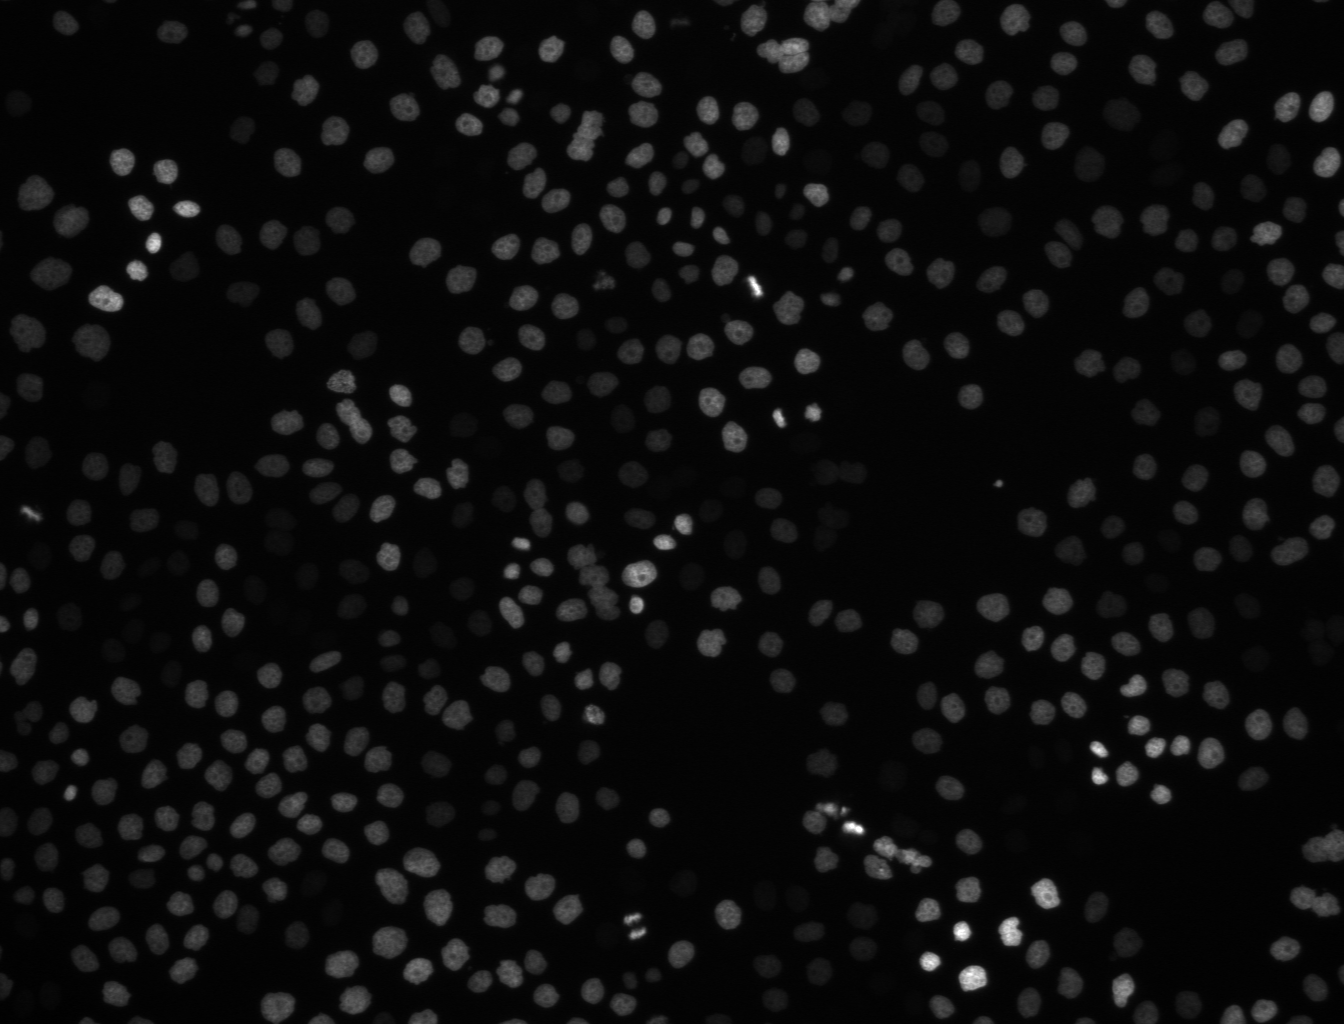
\includegraphics[width=\textwidth]{images/joint/overseg/75/raw.png}
        \caption{Raw data.}
    \end{subfigure}
    \hfill
    \begin{subfigure}[t]{0.48\textwidth}
        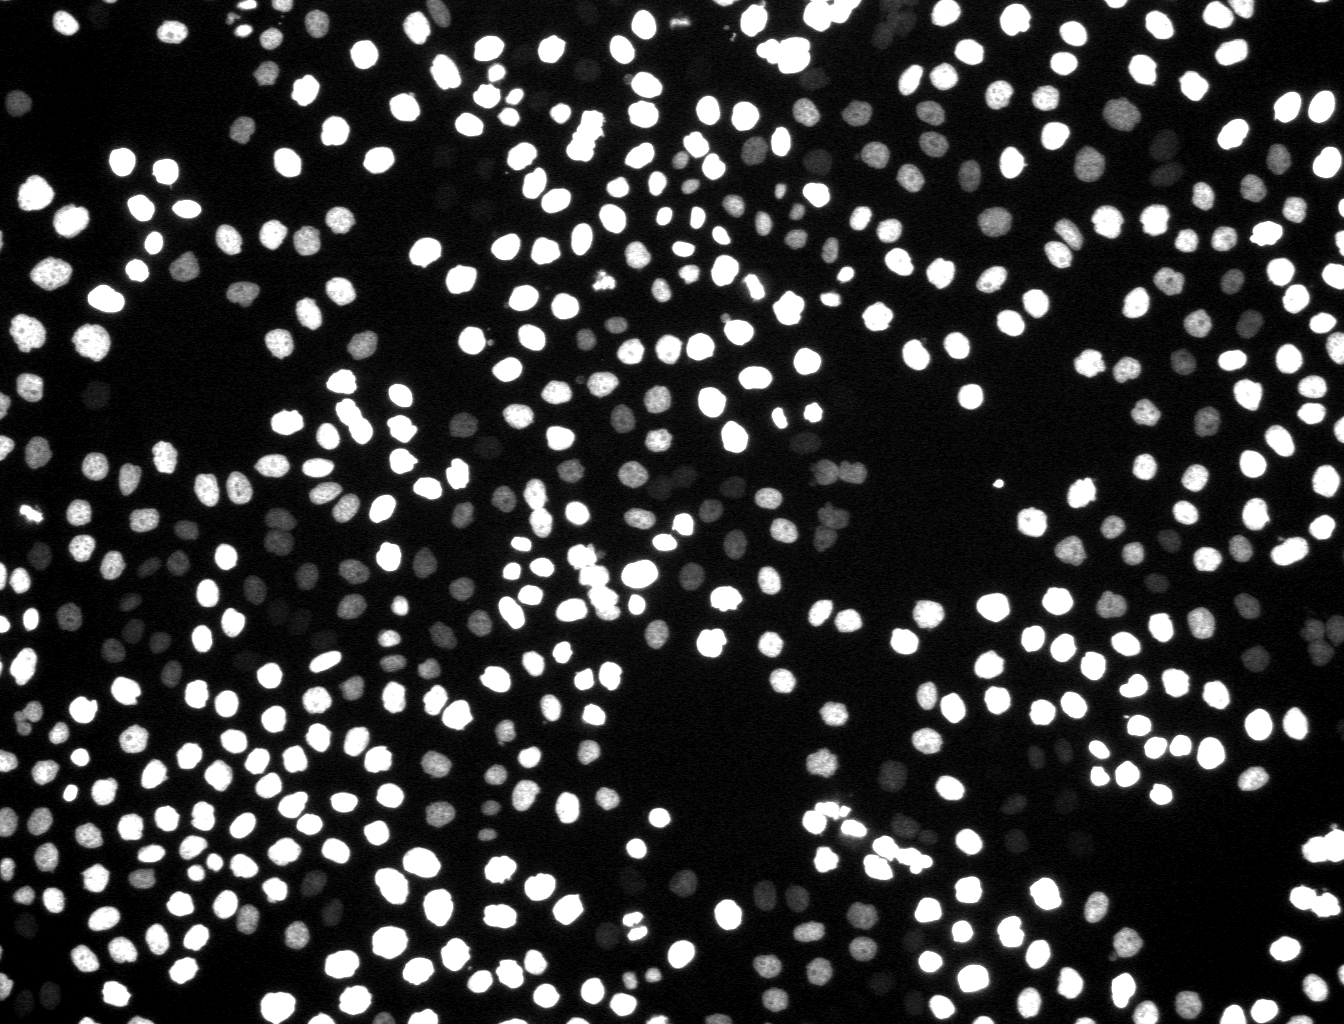
\includegraphics[width=\textwidth]{images/joint/overseg/75/raw_high_contrast.png}
        \caption{Raw data - enhanced contrast.}
    \end{subfigure}
    \\
    \begin{subfigure}[t]{0.48\textwidth}
        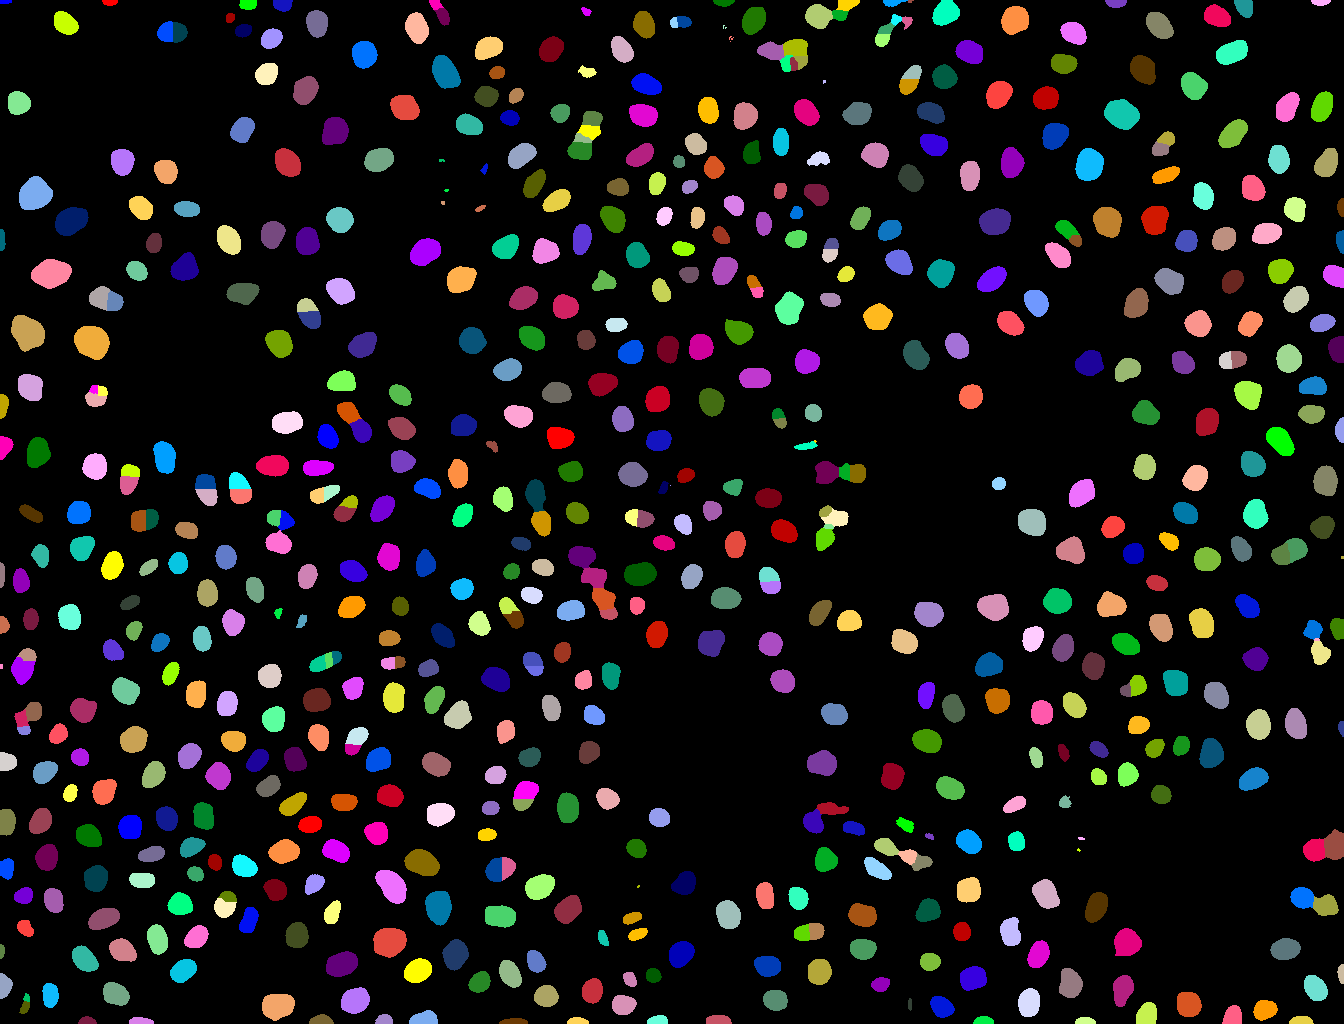
\includegraphics[width=\textwidth]{images/joint/overseg/75/colored.png}
        \caption{Initial oversegmentation.}
    \end{subfigure}
    \hfill
    \begin{subfigure}[t]{0.48\textwidth}
        \begin{tikzpicture}
            \node[anchor=south west,inner sep=0] (image) at (0,0)
            {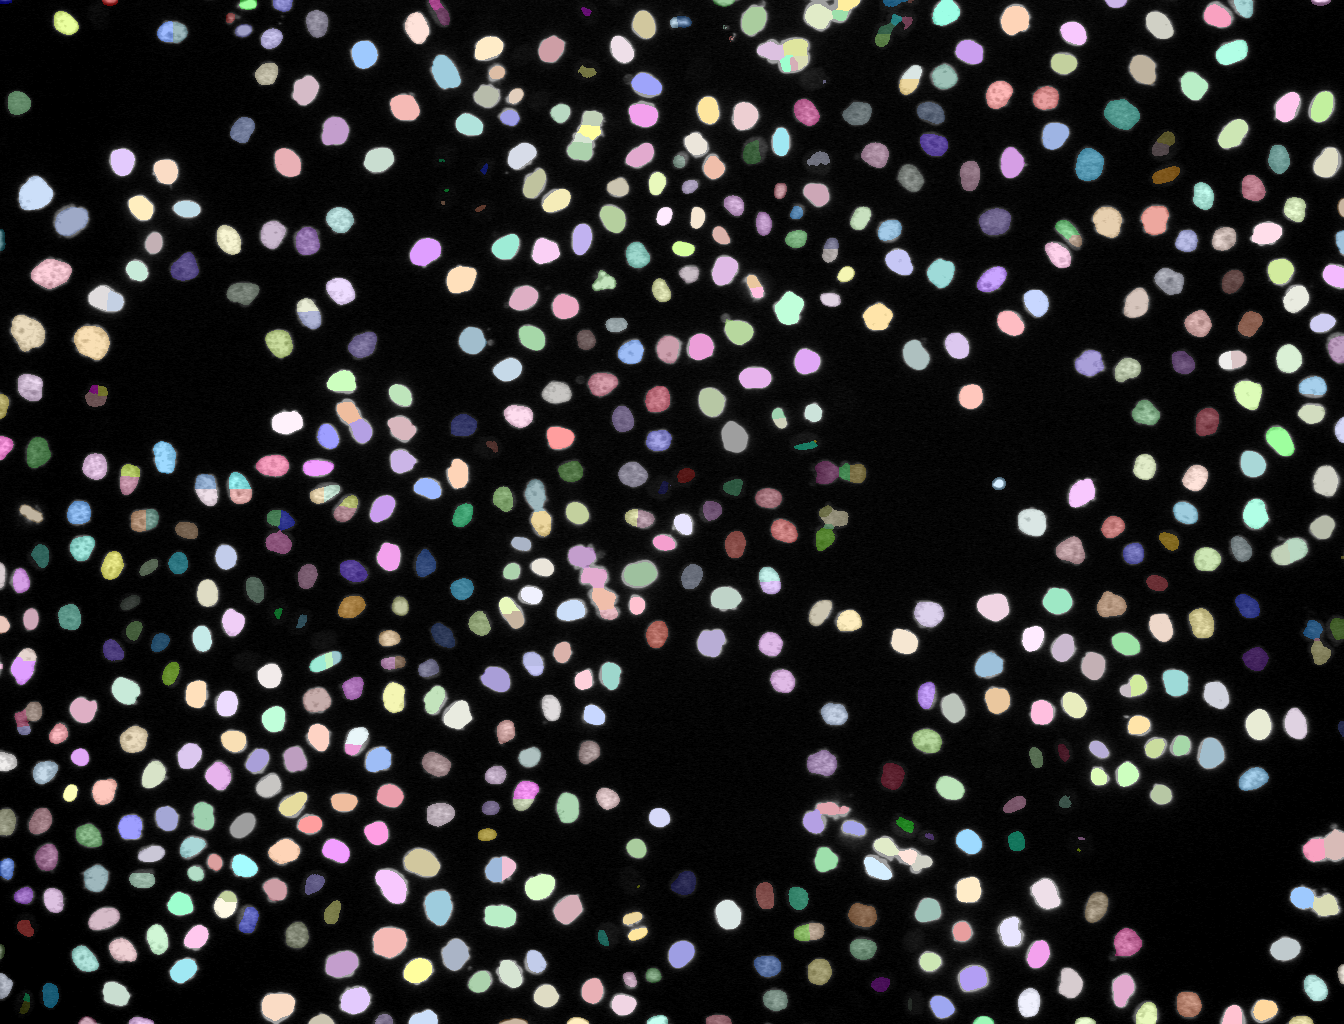
\includegraphics[width=\textwidth]{images/joint/overseg/75/overlay.png}};
            \begin{scope}[x={(image.south east)},y={(image.north west)}]
                \coordinate (c1) at (0.65,0.18);
                \coordinate (c2) at (0.69,0.16);
                \node[thick,draw,ellipse,fill opacity=0,color=magenta, fit=(c1) (c2), scale=0.4,
                xshift=1mm,yshift=-1mm] {};
                \coordinate (c3) at (0.8,0.17);
                \coordinate (c4) at (0.81,0.18);
                \node[thick,draw,ellipse,fill opacity=0,color=orange, fit=(c3) (c4), scale=0.5] {};
                \coordinate (c5) at (0.33,0.81);
                \coordinate (c6) at (0.36,0.83);
                \node[thick,draw,ellipse,fill opacity=0,color=orange, fit=(c5) (c6), scale=0.6] {};
            \end{scope}
        \end{tikzpicture}
        \caption{Overlay of the initial oversegmentation over raw data with enhanced contrast.}
    \end{subfigure}
    \caption[Initial oversegmentation for frame $75$ of data set C]{Initial oversegmentation for
        frame $75$ of data set C: For better distinguishability of the segments, a random color map
        has been applied to the segments in the bottom row.}
    \label{fig:joint-experiment-overseg-a}
\end{figure}

\begin{figure}
    \begin{subfigure}[t]{0.48\textwidth}
        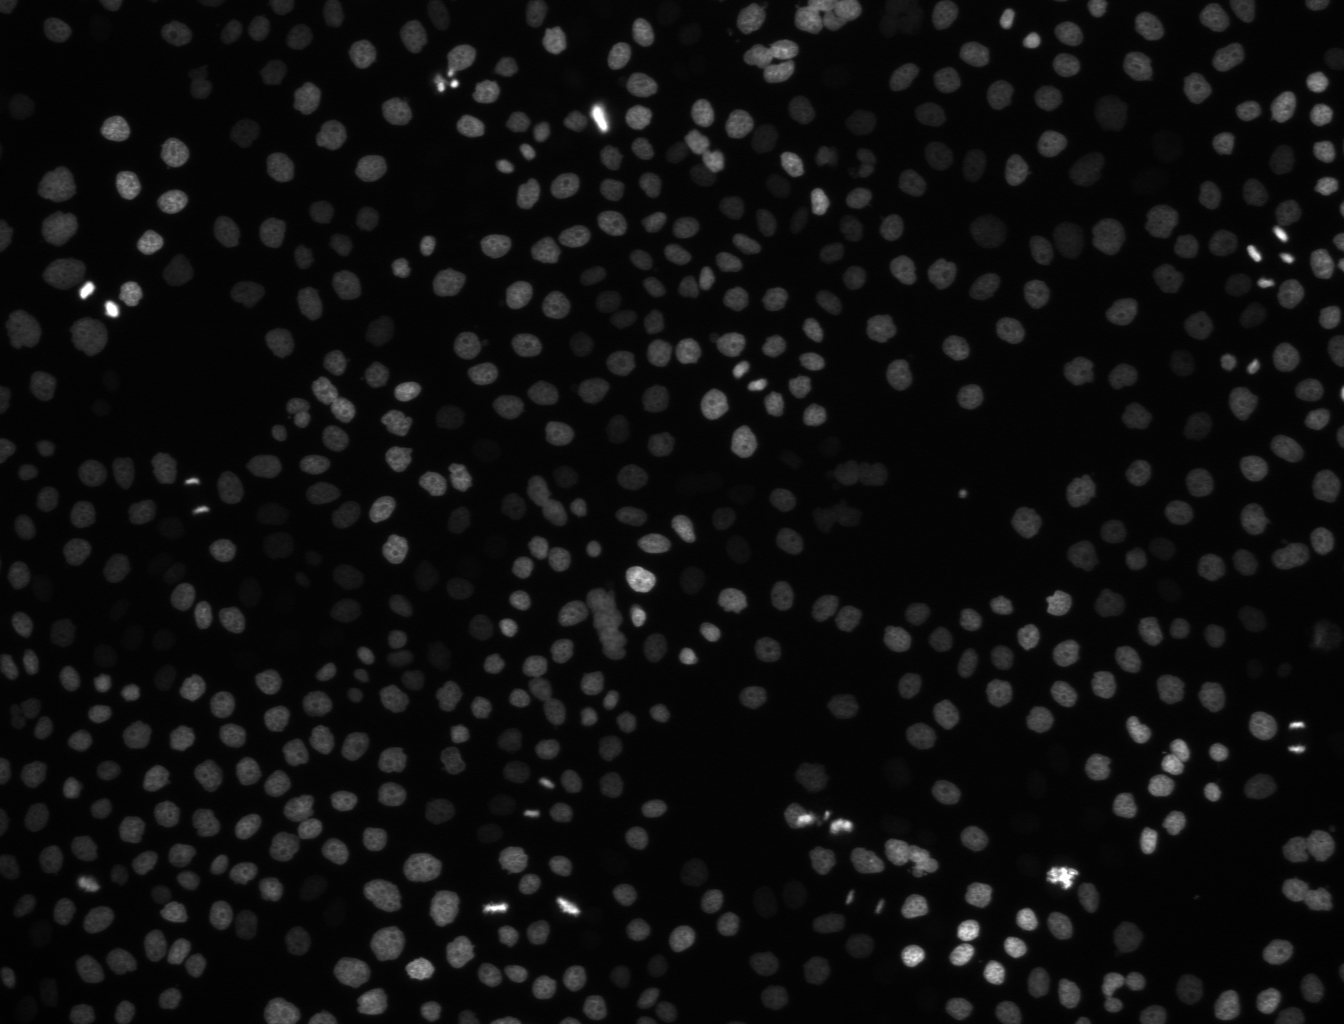
\includegraphics[width=\textwidth]{images/joint/overseg/85/raw.png}
        \caption{Raw data.}
    \end{subfigure}
    \hfill
    \begin{subfigure}[t]{0.48\textwidth}
        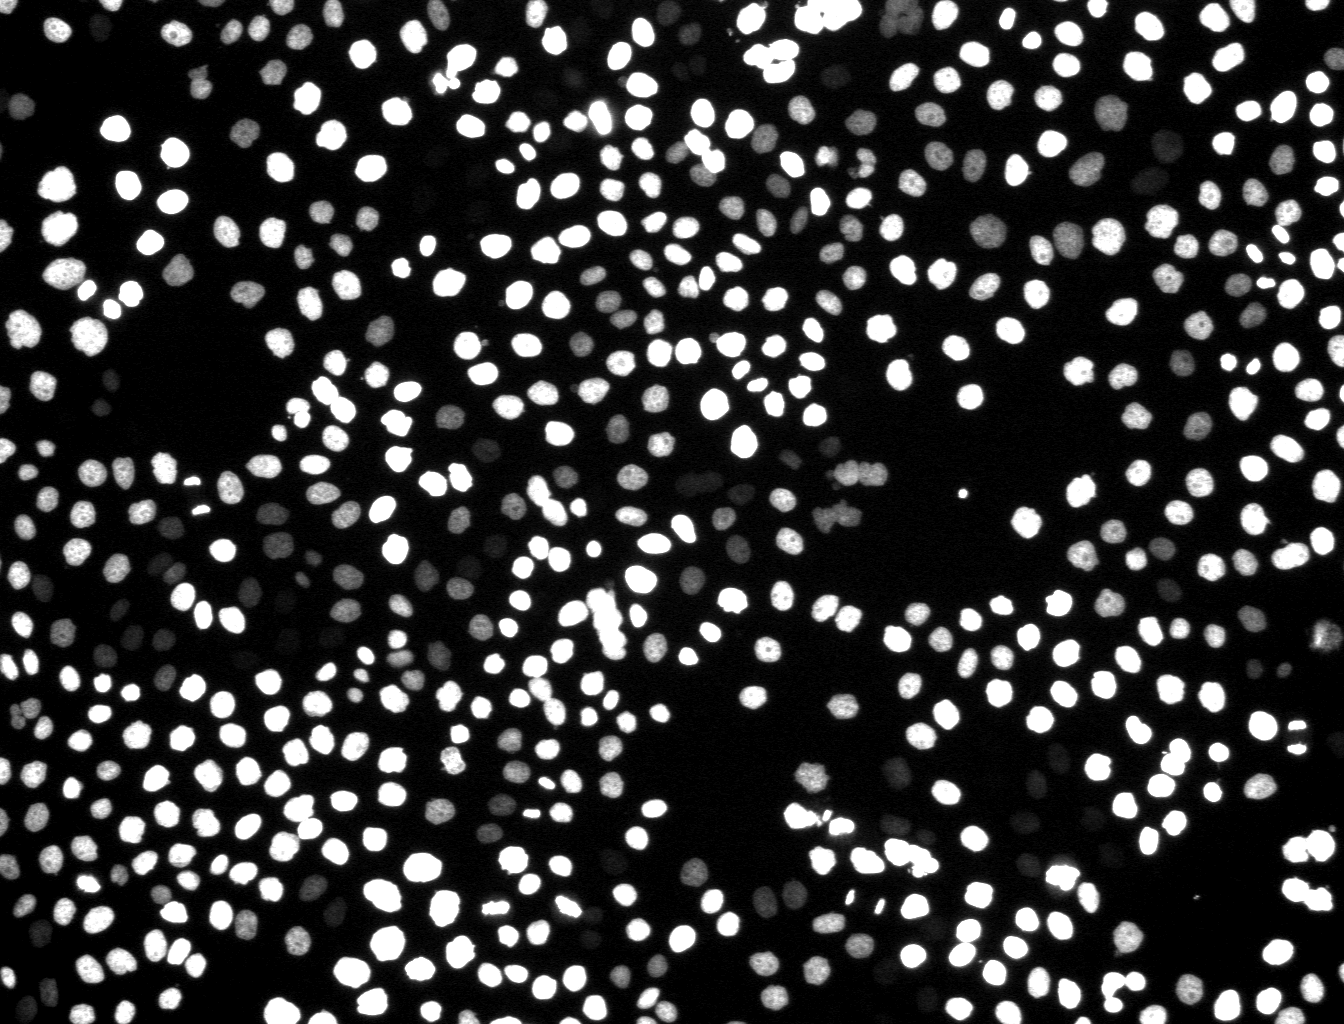
\includegraphics[width=\textwidth]{images/joint/overseg/85/raw_high_contrast.png}
        \caption{Raw data - enhanced contrast.}
    \end{subfigure}
    \\
    \begin{subfigure}[t]{0.48\textwidth}
        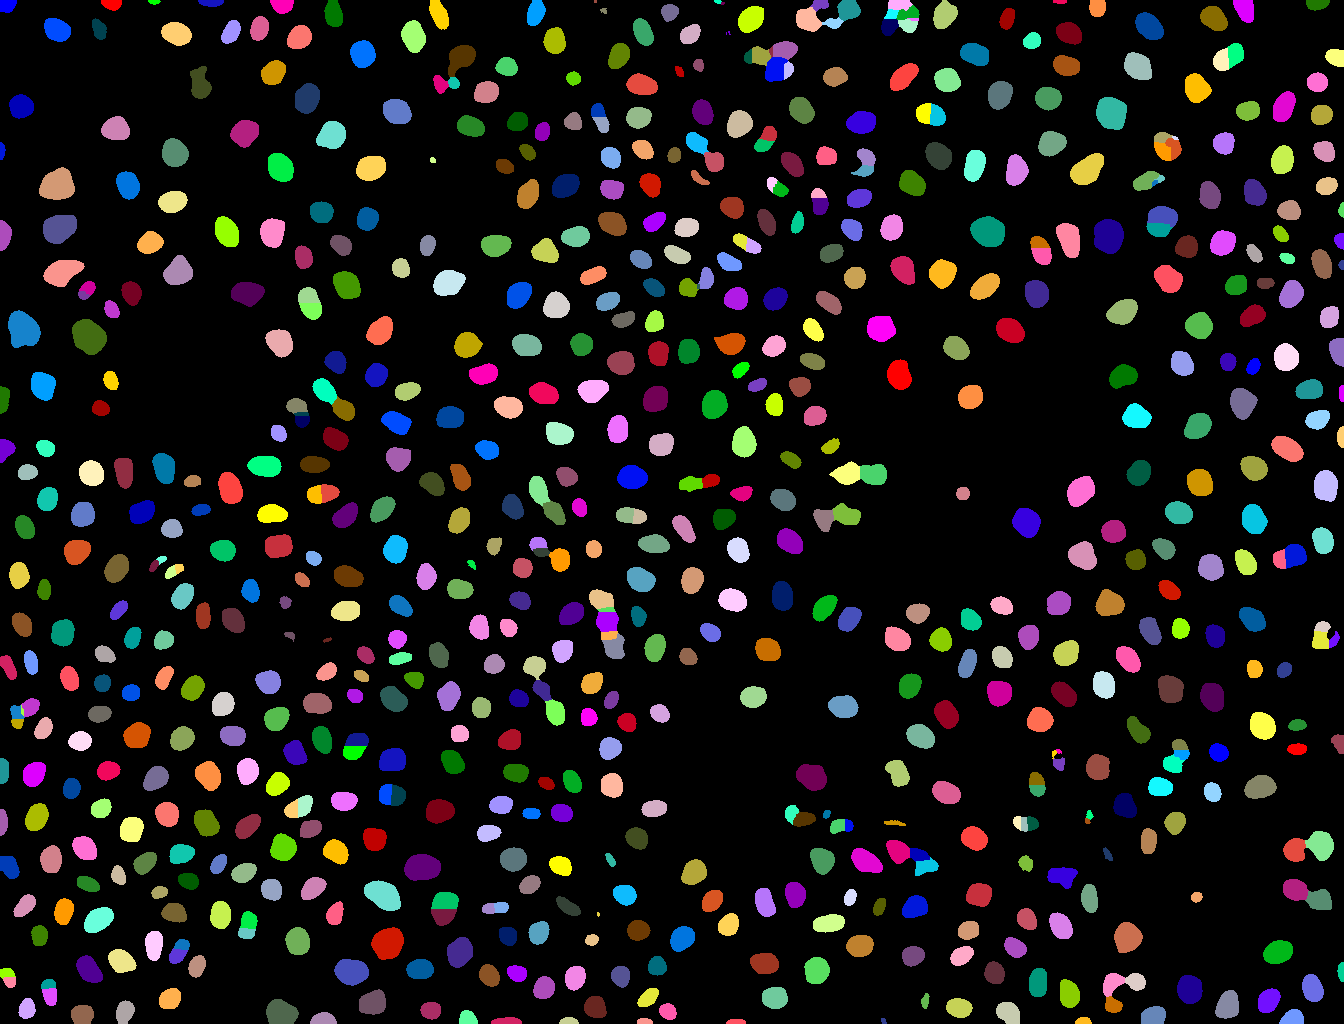
\includegraphics[width=\textwidth]{images/joint/overseg/85/colored.png}
        \caption{Initial oversegmentation.}
    \end{subfigure}
    \hfill
    \begin{subfigure}[t]{0.48\textwidth}
        \begin{tikzpicture}
            \node[anchor=south west,inner sep=0] (image) at(0,0)
            {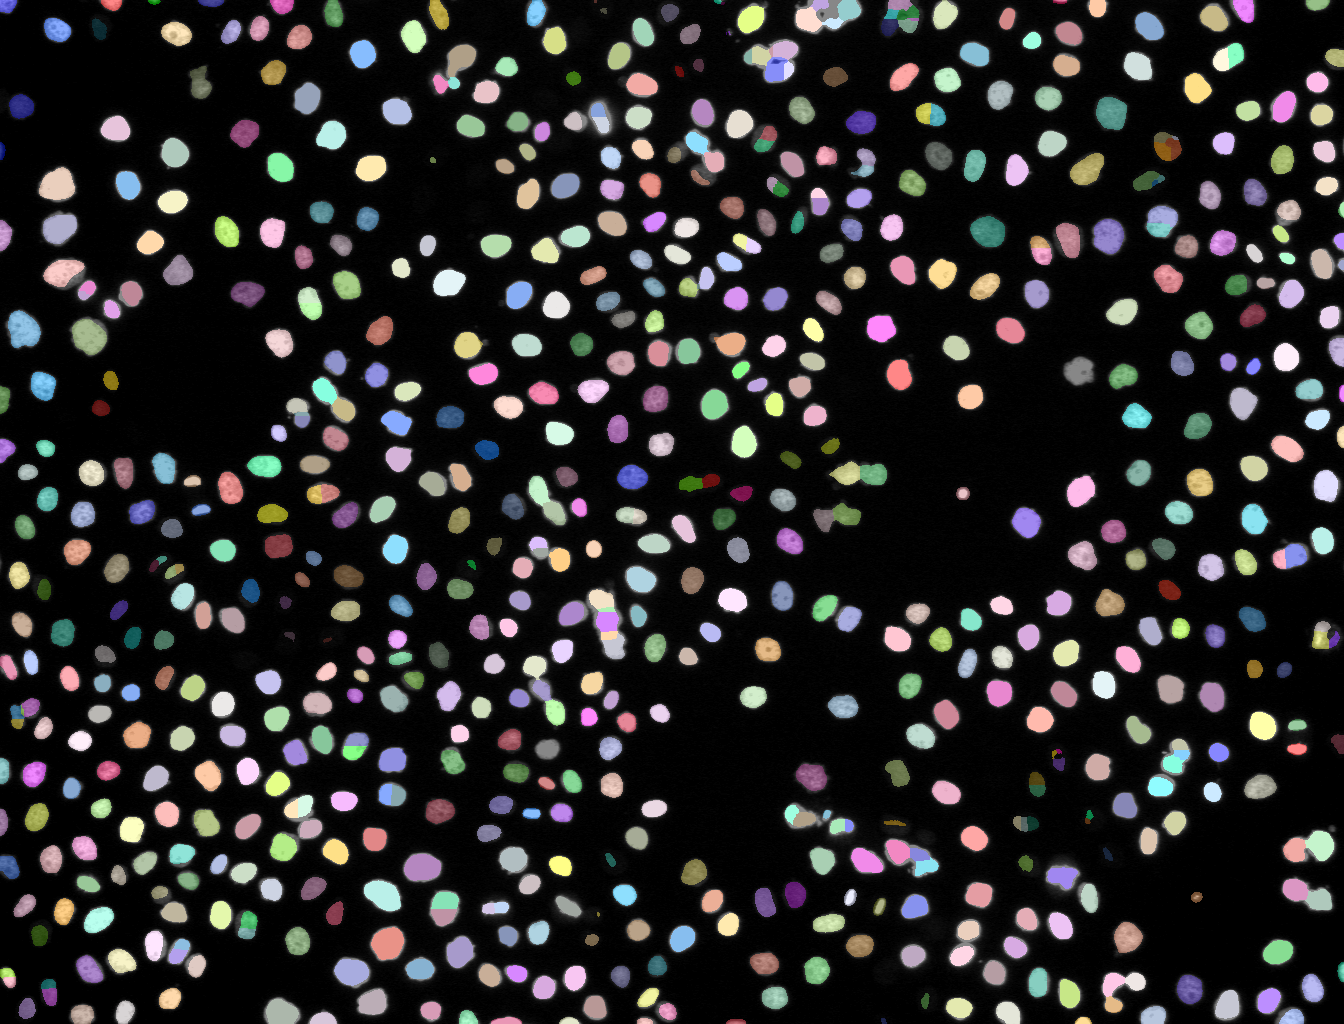
\includegraphics[width=\textwidth]{images/joint/overseg/85/overlay.png}};
            \begin{scope}[x={(image.south east)},y={(image.north west)}]
                % \draw[help lines,xstep=.1,ystep=.1] (0,0) grid (1,1);
                % \foreach \x in {0,2,...,8} { \node [anchor=north] at (\x/10,0) {0.\x}; }
                % \foreach \y in {0,2,...,8} { \node [anchor=east] at (0,\y/10) {0.\y}; }
                \coordinate (c1) at (0.87,0.25);
                \coordinate (c2) at (0.88,0.28);
                \node[thick,draw,ellipse,fill opacity=0,color=magenta, fit=(c1) (c2),scale=0.5,yshift=0mm] {};
                \coordinate (c3) at (0.445,0.105);
                \coordinate (c4) at (0.45,0.107);
                \node[thick,draw,ellipse,fill opacity=0,color=orange, fit=(c3) (c4),scale=0.35] {};
                \coordinate (c5) at (0.32,0.845);
                \coordinate (c6) at (0.325,0.855);
                \node[thick,draw,ellipse,fill opacity=0,color=orange, fit=(c5) (c6),scale=0.35,yshift=-1mm] {};
            \end{scope}
        \end{tikzpicture}
        \caption{Overlay of the initial oversegmentation over raw data with enhanced contrast.}
    \end{subfigure}
    \caption[Initial oversegmentation for frame $85$ of data set C]{Initial oversegmentation for
        frame $85$ of data set C: For better distinguishability of the segments, a random color map
        has been applied to the segments in the bottom row.}
    \label{fig:joint-experiment-overseg-b}
\end{figure}
Furthermore, while the merging algorithm not being sophisticated, the segments still are merged into
reasonable regions in the region merging~(\cf \cref{tab:joint-region-merging-examples}). Overall, the oversegmentation result forms
a legitimate basis for the subsequent tracking.
\begin{table}
    \centering
    \begin{tabular}{cccc}
        \toprule
        \multicolumn{1}{c}{Raw} & \multicolumn{1}{c}{Segments} & \multicolumn{1}{c}{Regions} & \multicolumn{1}{c}{Connected Component} \\ \midrule
        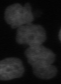
\includegraphics[width=0.15\textwidth]{images/joint/overseg/75/01/raw.png}
        & 
\includegraphics[width=0.15\textwidth]{images/joint/overseg/75/01/colored00.png}
        & 
\includegraphics[width=0.15\textwidth]{images/joint/overseg/75/01/colored01_all.png}
        & 
\includegraphics[width=0.15\textwidth]{images/joint/overseg/75/01/colored02.png} \\
        
\includegraphics[width=0.15\textwidth]{images/joint/overseg/75/02/raw.png}
        & 
\includegraphics[width=0.15\textwidth]{images/joint/overseg/75/02/colored00.png}
        & 
\includegraphics[width=0.15\textwidth]{images/joint/overseg/75/02/colored01_all.png}
        & 
\includegraphics[width=0.15\textwidth]{images/joint/overseg/75/02/colored02.png} \\
        % 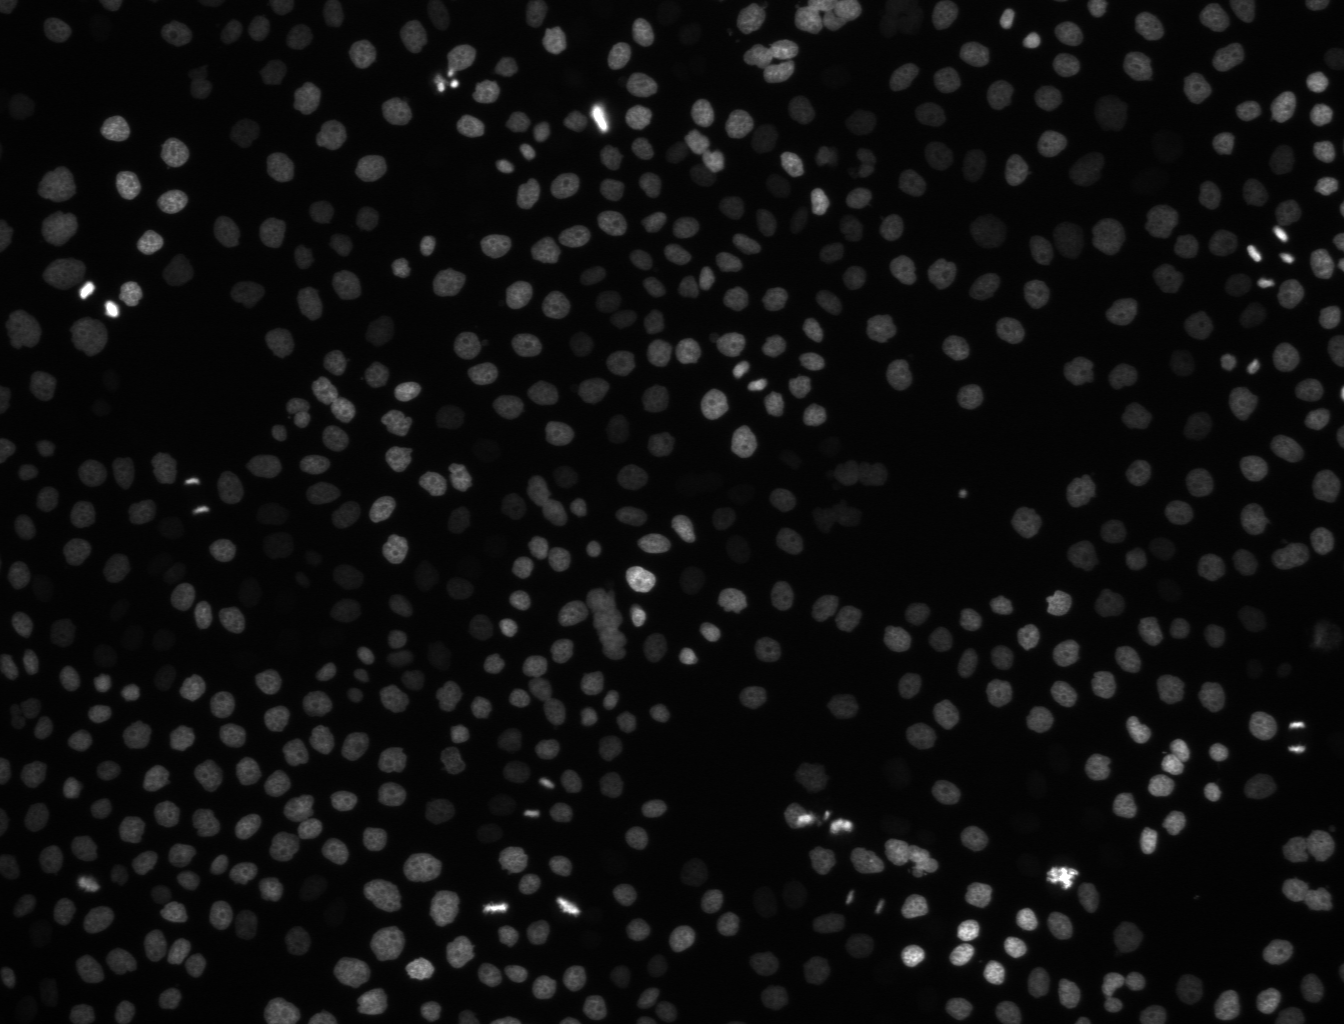
\includegraphics[width=0.15\textwidth]{images/joint/overseg/85/01/raw.png}
        % & 
\includegraphics[width=0.15\textwidth]{images/joint/overseg/85/03/colored00.png}
        % & 
\includegraphics[width=0.15\textwidth]{images/joint/overseg/85/03/colored01_all.png}
        % & 
\includegraphics[width=0.15\textwidth]{images/joint/overseg/85/01/colored02.png} \\
        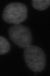
\includegraphics[width=0.15\textwidth]{images/joint/overseg/85/02/raw.png}
        & 
\includegraphics[width=0.15\textwidth]{images/joint/overseg/85/02/colored00.png}
        & % 
\includegraphics[width=0.15\textwidth]{images/joint/overseg/85/02/colored01_all.png}
        & 
\includegraphics[width=0.15\textwidth]{images/joint/overseg/85/02/colored01.png} \\
        \bottomrule
    \end{tabular}
    \caption[Region merging examples]{Region merging examples: The region merging reliably merges in
        a manner that forms new regions that are likely to be cells.  Here, a random color map is
        applied for better distinguishability of regions. If, like in the lowermost row
        where no intermediate regions exist,
        any merging would produce poor cell regions, no action is taken. The connected component is
        the union of all segments and is always a valid segmentation hypothesis by construction.}
    \label{tab:joint-region-merging-examples}
\end{table}



\subsubsection{Tracking Results}
\label{subsubsec:joint-experiment-tracking}
Three subsequent frames of the tracking result, based on the oversegmentation above, are shown in
\cref{fig:joint-tracking-result}. In general, the tracking result looks promising. When it comes to
challenging and more interesting connected components, however, the joint segmentation and tracking
fails. An example for this is indicated by a red ellipse in \cref{fig:joint-tracking-result} and
examined more closely in \cref{tab:joint-tracking-result}.
\begin{figure}
    \begin{subfigure}[t]{0.3\textwidth}
        \begin{tikzpicture}
            \node[anchor=south west,inner sep=0] (image) at(0,0)
            {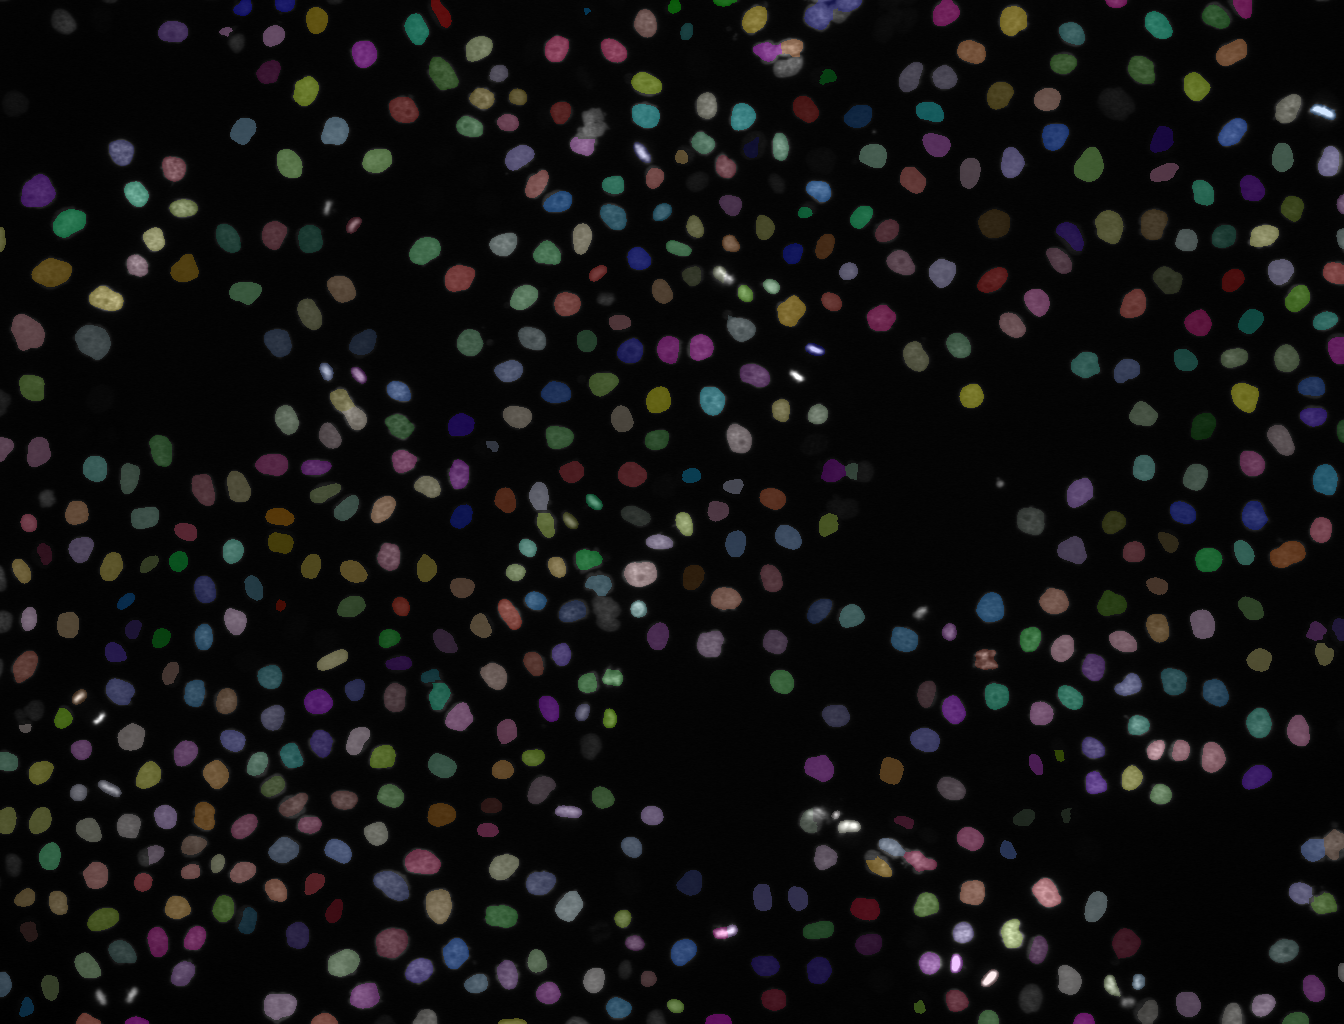
\includegraphics[width=1.0\textwidth]{images/joint/tracking/77_seg_overlay.png}};
            \begin{scope}[x={(image.south east)},y={(image.north west)}]
                \coordinate (c1) at (0.45,0.39);
                \coordinate (c2) at (0.45,0.44);
                \node[thick,draw,ellipse,fill opacity=0,color=red, fit=(c1)
                (c2),scale=0.4,yshift=-0.5mm, opacity=0.7] {};
            \end{scope}
        \end{tikzpicture}
        \caption{$t=77$}
    \end{subfigure}
    \hfill
    \begin{subfigure}[t]{0.3\textwidth}
        \begin{tikzpicture}
            \node[anchor=south west,inner sep=0] (image) at(0,0)
            {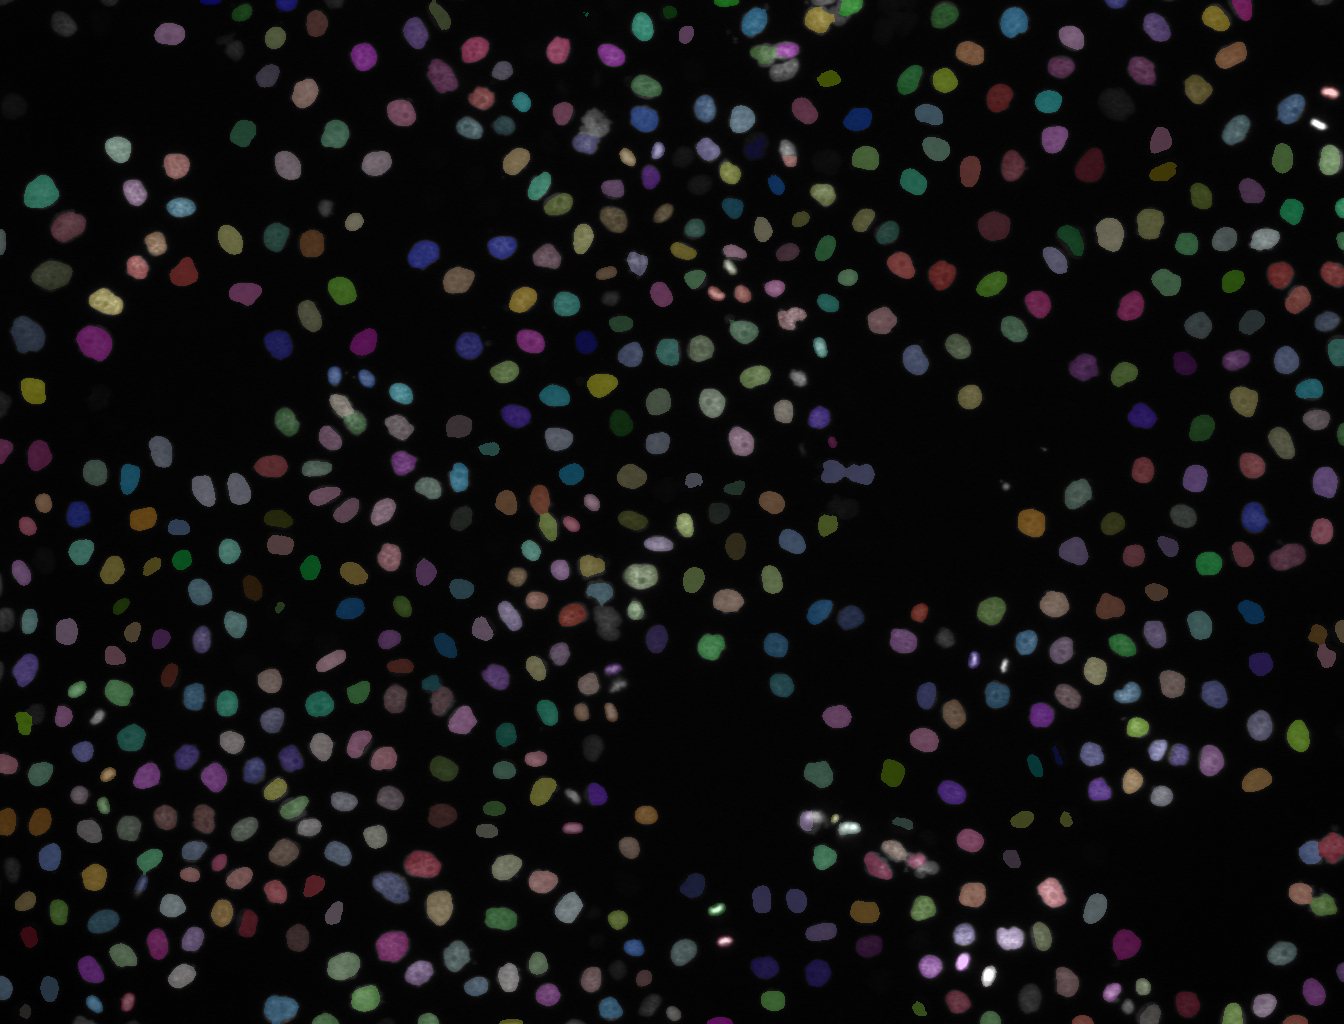
\includegraphics[width=1.0\textwidth]{images/joint/tracking/78_seg_overlay.png}};
            \begin{scope}[x={(image.south east)},y={(image.north west)}]
                \coordinate (c1) at (0.45,0.39);
                \coordinate (c2) at (0.45,0.44);
                \node[thick,draw,ellipse,fill opacity=0,color=red, fit=(c1)
                (c2),scale=0.4,yshift=-1.0mm, opacity=0.7] {};
            \end{scope}
        \end{tikzpicture}
        \caption{$t=78$}
    \end{subfigure}
    \hfill
    \begin{subfigure}[t]{0.3\textwidth}
        \begin{tikzpicture}
            \node[anchor=south west,inner sep=0] (image) at(0,0)
            {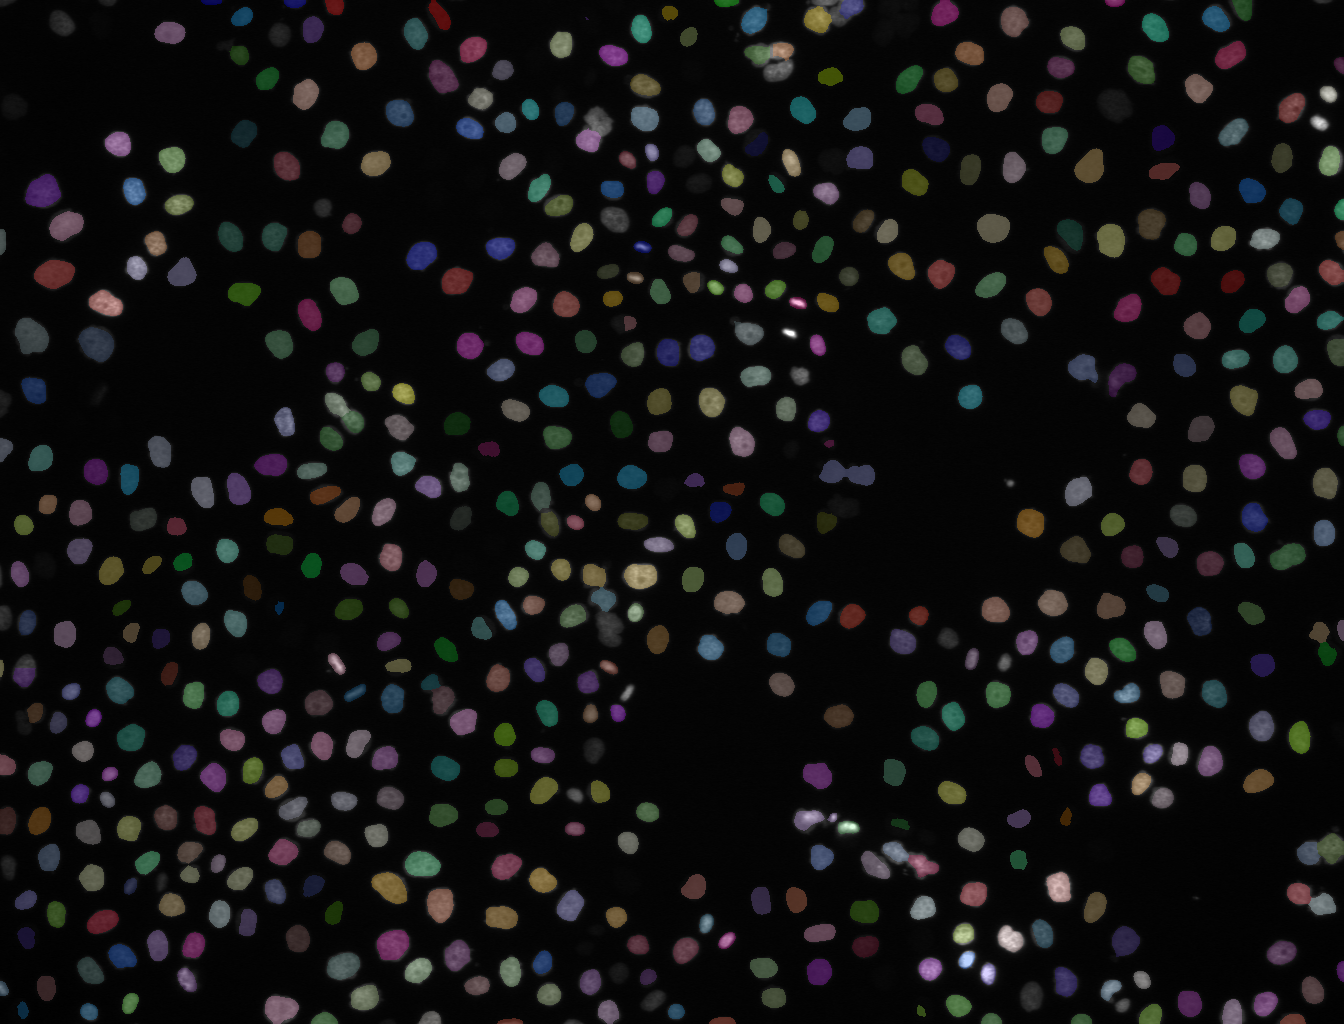
\includegraphics[width=1.0\textwidth]{images/joint/tracking/79_seg_overlay.png}};
            \begin{scope}[x={(image.south east)},y={(image.north west)}]
                \coordinate (c1) at (0.45,0.39);
                \coordinate (c2) at (0.45,0.44);
                \node[thick,draw,ellipse,fill opacity=0,color=red, fit=(c1)
                (c2),scale=0.4,yshift=-1.5mm, opacity=0.7] {};
            \end{scope}
        \end{tikzpicture}
        \caption{$t=79$}
    \end{subfigure}
    \\
    \begin{subfigure}[t]{0.3\textwidth}
        \begin{tikzpicture}
            \node[anchor=south west,inner sep=0] (image) at(0,0)
            {\includegraphics[width=1.0\textwidth]{images/joint/tracking/77_tracking_overlay.png}};
            \begin{scope}[x={(image.south east)},y={(image.north west)}]
                \coordinate (c1) at (0.45,0.39);
                \coordinate (c2) at (0.45,0.44);
                \node[thick,draw,ellipse,fill opacity=0,color=red, fit=(c1)
                (c2),scale=0.4,yshift=-0.5mm, opacity=0.7] {};
            \end{scope}
        \end{tikzpicture}
        \caption{$t=77$}
    \end{subfigure}
    \hfill
    \begin{subfigure}[t]{0.3\textwidth}
        \begin{tikzpicture}
            \node[anchor=south west,inner sep=0] (image) at(0,0)
            {\includegraphics[width=1.0\textwidth]{images/joint/tracking/78_tracking_overlay.png}};
            \begin{scope}[x={(image.south east)},y={(image.north west)}]
                \coordinate (c1) at (0.45,0.39);
                \coordinate (c2) at (0.45,0.44);
                \node[thick,draw,ellipse,fill opacity=0,color=red, fit=(c1)
                (c2),scale=0.4,yshift=-1.0mm, opacity=0.7] {};
            \end{scope}
        \end{tikzpicture}
        \caption{$t=78$}
    \end{subfigure}
    \hfill
    \begin{subfigure}[t]{0.3\textwidth}
        \begin{tikzpicture}
            \node[anchor=south west,inner sep=0] (image) at(0,0)
            {\includegraphics[width=1.0\textwidth]{images/joint/tracking/79_tracking_overlay.png}};
            \begin{scope}[x={(image.south east)},y={(image.north west)}]
                \coordinate (c1) at (0.45,0.39);
                \coordinate (c2) at (0.45,0.44);
                \node[thick,draw,ellipse,fill opacity=0,color=red, fit=(c1)
                (c2),scale=0.4,yshift=-1.5mm, opacity=0.7] {};
            \end{scope}
        \end{tikzpicture}
        \caption{$t=79$}
    \end{subfigure}
    \caption[Joint segmentation and tracking result for three consecutive frames:]{Joint
        segmentation and tracking result for three consecutive frames: $t=77$, $t=78$ and
        $t=79$. The bottom row shows the color coded tracking: In case of a division, the children
        cells take the color of their parent. This leads to ambiguities, when two cells with a
        common ancestor touch at a later stage in the tracking. With the colored tracking alone,
        this case cannot be distinguished from a wrong tracking where the two cells have been
        determined to be one larger cell. Therefore, the top row shows the active regions after
        inference. Here, the two cells in question have different color in case of a correct
        segmentation and tracking, and the same color otherwise. A typical tracking error is marked
        by a red ellipse.}
    \label{fig:joint-tracking-result}
\end{figure}

These illustrative examples have been picked because they demonstrate where joint segmentation and
tracking fails: In case of larger connected components with a higher number of segments, the
tracking tends to disable segments, even if inappropriate.

\newlength\tablemodifiermathheight
\settototalheight\tablemodifiermathheight{\parbox{\linewidth}{$71$}}
\begin{table}
    \centering
    \renewcommand*{\arraystretch}{0.5}
    \begin{tabular}{ccccc}
        $t$ & Raw & Oversegmentation & Connected Component & Tracking \\ \midrule
        $77$ & \raisebox{\tablemodifiermathheight-\height}{\includegraphics[width=0.15\textwidth]{images/joint/tracking/01/raw_crop.png}}
        & \raisebox{\tablemodifiermathheight-\height}{\includegraphics[width=0.15\textwidth]{images/joint/tracking/01/layer_00_crop.png}}
        & \raisebox{\tablemodifiermathheight-\height}{\includegraphics[width=0.15\textwidth]{images/joint/tracking/01/layer_04_all_crop.png}}
        &
        \raisebox{\tablemodifiermathheight-\height}{\includegraphics[width=0.15\textwidth]{images/joint/tracking/01/77_tracking_overlay_crop.png}}
        \\ &&&& \\
        $78$ & \raisebox{\tablemodifiermathheight-\height}{\includegraphics[width=0.15\textwidth]{images/joint/tracking/02/raw_crop.png}}
        & \raisebox{\tablemodifiermathheight-\height}{\includegraphics[width=0.15\textwidth]{images/joint/tracking/02/layer_00_crop.png}}
        & \raisebox{\tablemodifiermathheight-\height}{\includegraphics[width=0.15\textwidth]{images/joint/tracking/02/layer_04_all_crop.png}}
        &
        \raisebox{\tablemodifiermathheight-\height}{\includegraphics[width=0.15\textwidth]{images/joint/tracking/02/78_tracking_overlay_crop.png}}
        \\ &&&& \\
        $79$ & \raisebox{\tablemodifiermathheight-\height}{\includegraphics[width=0.15\textwidth]{images/joint/tracking/03/raw_crop.png}}
        & \raisebox{\tablemodifiermathheight-\height}{\includegraphics[width=0.15\textwidth]{images/joint/tracking/03/layer_00_crop.png}}
        & \raisebox{\tablemodifiermathheight-\height}{\includegraphics[width=0.15\textwidth]{images/joint/tracking/03/layer_04_all_crop.png}}
        &
        \raisebox{\tablemodifiermathheight-\height}{\includegraphics[width=0.15\textwidth]{images/joint/tracking/03/79_tracking_overlay_crop.png}}
        \\ &&&& \\
        \bottomrule 
    \end{tabular}
    \renewcommand*{\arraystretch}{1.0}
    \caption[A single connected component with falsely deactivated regions]{A single connected component with falsely deactivated regions (no intermediate regions
        were merged from the segments). The same cluster of cells is shown over three time steps with the according segmentation showing that an
        activation of more regions would have been reasonable. However, the factor graph decided to
        turn off some of the cell-like regions. In an optimal tracking, the lower part of the merged
        object in the middle would be active.}
    \label{tab:joint-tracking-result}
\end{table}

% In addition and due to the lack of a gold standard, the tracking result has been evaluated by manual
% inspection. A random selection of events both in ground truth and tracking result form the basis for
% comparison. The results are summarized in \cref{tab:joint-result-numbers}.
The ground truth used for evaluation of the conservation tracking method in
\cref{sec:gmm-experiments} is based on the segmentation that was used for tracking and thus cannot
be used as a gold standard in the joint tracking and segmentation.  Therefore,
\cref{tab:joint-result-numbers} shows the results of a manual evaluation of a selection of cells
compared to raw data by visual inspection. For that purpose, $317$ moves have been randomly selected
from each of raw data and tracking result. For the divisions, a random subset of $100$ and $87$
events has been picked from tracking result and raw data, respectively. Randomness is injected by
random sampling from the events on the tracking result side, and by choosing the event that is
closest to a randomly sampled tuple of time step and coordinates in case of raw data events.

In a strict measure for move events, moves are considered false moves if they connect regions that
either exceed one and a half times of, or fall below half the size of the corresponding cell in raw
data. On the contrary, in a relaxed measure, these moves fall in the true positive category, \cf the
rows starting with \emph{Moves} in \cref{tab:joint-result-numbers}. Similarly, divisions are off by
one or two time steps compared to raw data in many cases. Therefore, an additional, more tolerant
measure for divisions is applied, which considers a division true positive, if the
corresponding raw data division occurs within a range of two time steps, \cf the rows starting with
\emph{Divisions} in \cref{tab:joint-result-numbers}. Note that, in contrast to mitosis detection and
without exception, a division is only true positive, if all three involved cells, \ie parent and
child cells, are detected correctly.



The results in \cref{tab:joint-result-numbers} confirm that the overall tracking result looks
promising. The lower recall for moves in comparison to precision indicates that the tracking falsely
deactivates too many regions. Furthermore, the discrepancy between strict and tolerant division
measures implies that a better division classifier could improve tracking results. Still, even with
the more tolerant measures, there is room for improvement, as the aforementioned problem of falsely
deactivated regions persists. In the following, we identify the reasons for these shortcomings and
justify future work and enhancement of the model.

\begin{table}
    \centering
    \begin{tabular}{l|ccc}
        \toprule
        & Precision & Recall & $\fmeasure$ \\ \hline
        Moves - size filter\tablefootnote{A move is only true positive if both involved regions are larger
            than half the size and smaller than 1.5 times the size of the the cell in raw data.} & 0.970 & 0.901 & 0.934 \\
        Moves - no size filter\tablefootnote{The size filter for regions that are involved in moves
            is not applied.} & 0.979 & 0.921 & 0.949 \\
        Divisions - strict\tablefootnote{If a division occurs at a time shifted by one or two compared to
            raw data, it is considered a wrong event.} & 0.654 & 0.654 & 0.654 \\
        Divisions - tolerant\tablefootnote{Divisions have a time step tolerance of $2$.} & 0.890 & 0.825
        & 0.856 \\
        \bottomrule
    \end{tabular}
    \caption[Joint segmentation and tracking results]{Joint segmentation and tracking results for
        data set C (\cref{subsec:gmm-data}) based
        on evaluation by visual inspection. Precision, recall and $\fmeasure$
        (\cref{subsec:gmm-measures}) are used for evaluation of the data. We present both strict and more
        tolerant evaluation schemes for moves and divisions.}
    \label{tab:joint-result-numbers}
\end{table}



\subsection{Continuation of the Work on the Model}
\label{subsec:joint-continuation}
As demonstrated in the previous sections, joint segmentation and tracking suffers from tracking
errors in the presence of connected components with many segments. More specifically, regions
corresponding to actual cells are deactivated in the tracking. However, the active regions in the
final result still constitute a meaningful tracking with the limitation that divisions appear one or
two time steps too early in many cases. Thus, the task for ongoing work on the model is to modify
the method in a way that pushes the result towards activating these falsely deactivated regions.

Due to the complexity of the method, locating the weak spots is essential. To begin with, the
initial oversegmentation seems reasonable. As demonstrated in
\cref{fig:joint-experiment-overseg-a,fig:joint-experiment-overseg-b}, the initial segments
either oversegment or exactly fit single cells in most cases. Furthermore,
\cref{tab:joint-region-merging-examples} shows that the region merging works well by producing a
richer set of cell-like regions. A more sophisticated merging algorithm would not fundamentally
change the tracking result. However, learned edge weights based on the output of the region
classifier~(\cref{sec:joint-classifier-Region}) could easily be implemented into the workflow
and would give a more reasonable basis for the classifier decision.

On the other hand, the factor graph wrongly decided to turn off regions and, in many cases,
inferred divisions one time step too early. Thus the error occurs in the creation of the
hypotheses or during inference and these steps need to be revised with the following approaches
promising positive results:

To begin with, the pruning of potential assignments (\cref{subsec:joint-hypotheses-graph}) may be too
restrictive and discard assignment hypotheses, which would have turned out to be true. Take two
connected components $c^t$ and $c^{t+1}$ at times $t$ and $t+1$, respectively, each consisting
of two segments. If the displacement of the connected components is large enough, both conflict
sets in $c^t$ might have the same conflict set in $c^{t+1}$ for their nearest neighbor. In that
case, inference would tend to falsely disable regions without incoming assignment hypotheses,
even if it contradicts the actual events in raw data. A solution to this problem could be a less
restrictive pruning algorithm. This could be achieved by finding more than one nearest neighbors
for each conflict set. However, with a nearest neighbor search only in forward direction in
time, the potential loss of regions persists. Therefore, a single nearest neighbor should be
searched both forward and backward in time. In this, all regions have incoming assignment
hypotheses, unless the encompassing connected component does not have any incoming arcs in the
hypotheses graph.

Moreover, the division classifiers tend to predict divisions one time step too early. The obvious
answer to this issue is a retraining of the division classifiers. For a definite evaluation of the
classifiers, their output needs to be visualized. Due to the prediction for all possible divisions
of a cell, this turns out unmanageable. A reasonable approximation is the probability of the most
likely division. In the corresponding visualization, cells take values according to the maximum
division probability. With an appropriate color map, \eg gray scale or jet\footnote{Low and high
    values are represented by blue and red color, respectively,
    \\\cf\url{http://wiki.scipy.org/Cookbook/Matplotlib/Show_colormaps}.}, the classifier prediction
can be efficiently compared to the tracking result and the source of the early divisions can be
located at either of the division classifier or the graphical model.

Finally, bugs in the code cannot be excluded as a source for problems. Thus a revision of the code
is necessary. In order to analyze the behavior of the model and the effects of potential solutions
to the existing problems, and to fix potential bugs, a small subset of representative cells should
be cropped from raw data. The sample should be sufficiently small to allow for a manual reproduction
of the factor graph and inference. Furthermore, these examples with the desired results should serve
as unit tests in addition to existing ones.

A more radical approach would be a complete revision of the graphical model in conjunction with a
disposal of the region merging. Then, based on the initial oversegmentation, the graphical model
would decide, which segments should be merged into larger regions. This, however, would require
multi-state random variables and higher order factors that manage the grouping of segments into
larger regions and enforce additional consistency constraints, \eg regions must be connected. In
addition to this explosion of the model, the labeling would be ambiguous: Labeling one region $1$
and another region $2$ is equivalent to setting the labels the other way round. Therefore, although
this approach is really interesting in theory, in practice it would not be tractable. An even more
extreme effort would be a complete omission of the initial segmentation and building the factor
graph on the pixel level. However, it is obvious that this problem is not tractable by any means due
to its huge size.

In summary, we proposed a method that jointly optimizes segmentation and tracking as an approach to
handle undersegmentation in cell tracking, and thereby goes beyond existing tracking-by-assignment
methods~(\cref{fig:joint-pipeline}). First, a set of possibly competing segmentation hypotheses is
generated~(\cref{sec:joint-oversegmentation}). Then, the factor graph chooses those segmentations
that constitute the most meaningful tracking result~(\cref{sec:joint-graphical-model}). To this end,
discriminative classifiers for count, regions, divisions and moves~(\cref{sec:joint-classifiers})
implement local evidence in the factors. Finally, experiments in \cref{sec:joint-experiments} show
promising results that suggest a continuation of the work on the model in order to solve the
existing issues~(\cref{subsec:joint-continuation}).

%%% Local Variables: 
%%% mode: latex
%%% TeX-master: "../../../main"
%%% End: 



%%% Local Variables: 
%%% mode: latex
%%% TeX-master: "../../main"
%%% End: 
